%-*-    coding: UTF-8   -*-
% !TEX program = xelatex
\documentclass[UTF-8]{ctexart}
\usepackage{array}
\usepackage{graphicx}
\usepackage{float}
\usepackage{subfigure}
\usepackage{amsmath}
\usepackage{amssymb}
\usepackage{tabularx}
\usepackage{multirow}
\usepackage[usenames,dvipsnames]{color}
\usepackage{framed}
\usepackage{xcolor}
\usepackage{hyperref}
\usepackage{verbatim}
\hypersetup{
	colorlinks=true,
	linkcolor=black,
	filecolor=black,
	urlcolor=blue,
	citecolor=black,
}
\usepackage{ulem}
\usepackage[cache=false]{minted}
\setminted{tabsize=4}
\usepackage{geometry}
\geometry{a4paper,centering,scale=0.85}
\usepackage[format=hang,font=small,textfont=it]{caption}
\usepackage[nottoc]{tocbibind}

\definecolor{LightofNibel}{rgb}{0.6,0.85,0.95}
\pagecolor{white}

\title{\textbf{\huge 给信息组学弟学妹的 Linux 入门手把手教程}}
\author{\texttt{iotang}}
%\date{}

\begin{document}
	\maketitle
	
	\begin{figure}[H]
		\centering
		\begin{minipage}{0.15\textwidth}
			\centering
			
\includegraphics[width=\textwidth]{fig/cj.png}
			\caption*{}
		\end{minipage}
		\begin{minipage}{0.15\textwidth}
			\centering
			
\includegraphics[width=\textwidth]{fig/iotang_victini.jpg}
			\caption*{}
		\end{minipage}
		\begin{minipage}{0.15\textwidth}
			\centering
			
\includegraphics[width=\textwidth]{fig/tux.png}
			\caption*{}
		\end{minipage}
		\begin{minipage}{0.15\textwidth}
			\centering
			
\includegraphics[width=\textwidth]{fig/ubuntu.png}
			\caption*{}
		\end{minipage}
		\\
		\textit{本文的 4 个要素}
	\end{figure}

	\newpage
	
	\vspace*{\fill}
	\begin{center}
		{\large
		本作品所有内容采用\href{http://creativecommons.org/licenses/by-sa/4.0}{知识共享署名-相同方式共享 4.0 国际许可协议}进行许可,
		
		以兼容 GNU LESSER GENERAL PUBLIC LICENSE Version 3 协议。
		}
		\begin{figure}[H]
			\centering
			\begin{minipage}{0.15\textwidth}
				\centering
				
\includegraphics[width=\textwidth]{fig/cc.xlarge.png}
				\caption*{}
			\end{minipage}
			\begin{minipage}{0.15\textwidth}
				\centering
				
\includegraphics[width=\textwidth]{fig/by.xlarge.png}
				\caption*{}
			\end{minipage}
			\begin{minipage}{0.15\textwidth}
				\centering
				
\includegraphics[width=\textwidth]{fig/sa.xlarge.png}
				\caption*{}
			\end{minipage}
		\end{figure}
		
	\end{center}
	\vspace*{\fill}
	
	\newpage
	
	\tableofcontents

	\newpage

	\section{欢迎使用 Linux!}
	
		学弟学妹们好!感谢你们参加信息学竞赛!
		
		比克提尼 iotang 在这里献上最诚挚的祝福!
			
		\begin{figure}[H]
			\centering
			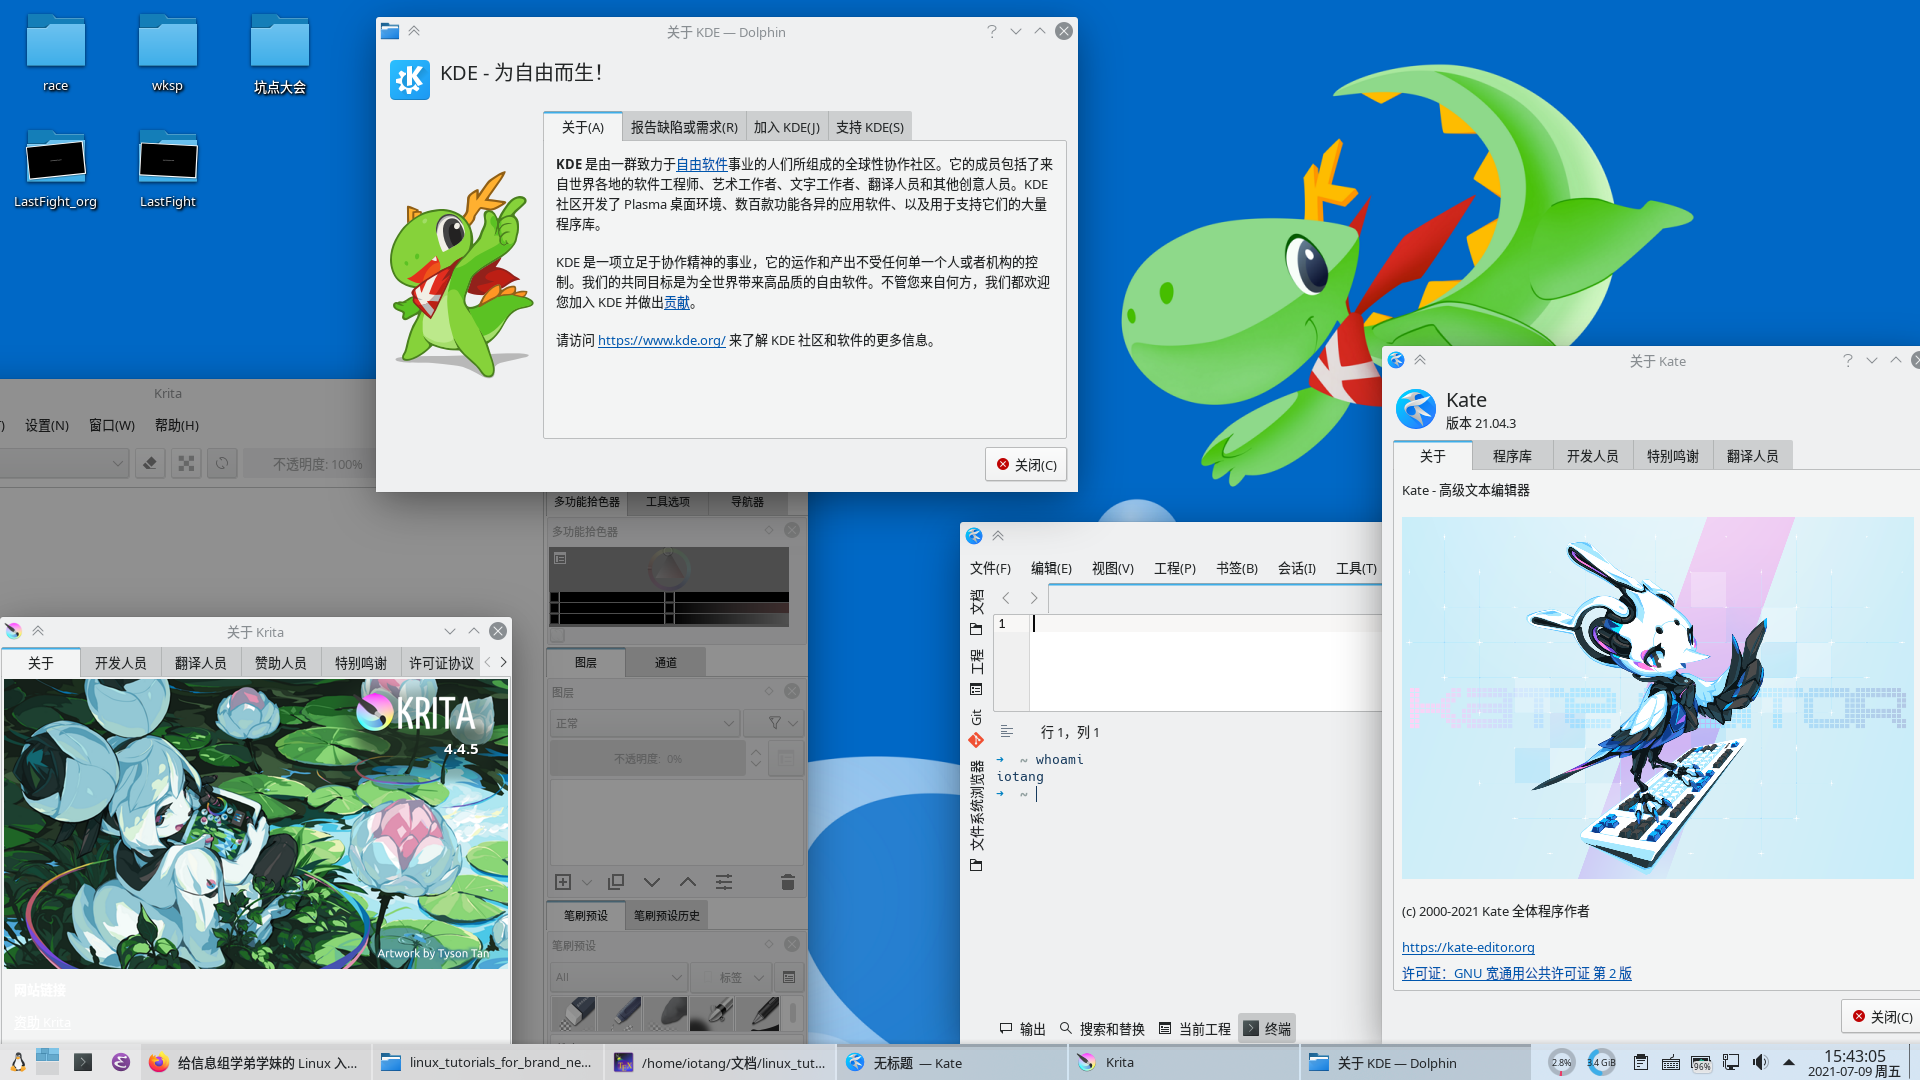
\includegraphics[width=0.8\textwidth]{fig/iotangsdesktop.png}
			\caption*{iotang 与 Konqi(左上、右上)、Kiki(左下)和 Kate(右下)向你发出问候}
		\end{figure}
	
		大家应该都对 Linux 有所耳闻,不过我猜有许多人都以为 Linux 很难用、不好用而不敢迈出第一步。
		
		现在,就让我来手把手带你们入门 Linux!
	
		\subsection{Linux 是开源软件}
		
			Linux 遵循 GNU 通用公共许可证,任何人都可以自由使用它的源代码。
			
			(注意,这里并没有说 Linux 是“不要钱”地使用的,不过既然你都可以搞到源代码了,那么收费基本也就没必要了。不过还是有服务以付费的方式给出。)
			
			\begin{figure}[H]
				\centering
				
\includegraphics[width=0.3\textwidth]{fig/tux.png}
				\caption*{Linux 的吉祥物 Tux}
			\end{figure}
			
		\subsection{为什么是 Ubuntu?}
		
			Ubuntu 是 Linux 操作系统中的一种。接下来给大家带来的 Linux 教程主要是以 Ubuntu 为平台来实现的。
		
			首先很明显的是,NOI Linux 就是一个换皮的 Ubuntu。至于为什么是 Ubuntu,可能与 Ubuntu 在中国的强大的用户数量有关。
			
			用户多教程就多,问题解决也方便,\sout{不像笔者硬是要搞个 Arch Linux 然后折腾}。
			
			所以说,从竞赛与使用方面,这边还是建议大家用 Ubuntu。
		
			\begin{figure}[H]
				\centering
				
\includegraphics[width=0.3\textwidth]{fig/ubuntu.png}
				\caption*{Ubuntu 的标志}
			\end{figure}
		
	\newpage
	
	\section{Ubuntu 的安装}
	
		\subsection{下载镜像文件}
		
			非常简单,你只要先百度 ubuntu,进入官网(注意:有中文官网),然后进入下载栏目下载就可以了。
			
			\subsubsection{我该选哪一个?}
			
				在下载界面你可以发现一些不同版本:
				
				\begin{figure}[H]
					\centering
					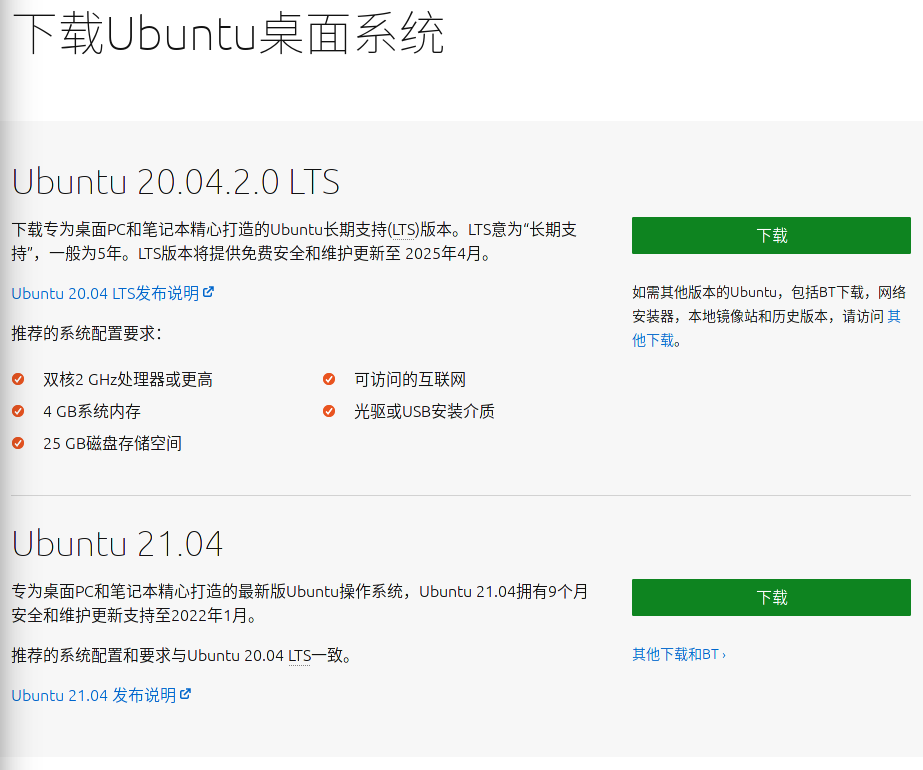
\includegraphics[width=0.8\textwidth]{fig/download_ubuntu_which.png}
					\caption*{两种选择}
				\end{figure}
			
				其中,带“LTS”的版本意为长期支持版本,有 5 年的免费安全和维护更新时间;而不带 LTS 的一般只维护 9 个月,因为带 LTS 的版本每 2 年发布一个,而不带 LTS 的每半年就发布一个,你需要及时更新。
				
				这里为了稳定性,我们下载那个带 LTS 的版本。
			
			\subsubsection{下载的速度太慢了?}
			
				你可以去其它的镜像网站。这里以网易开源镜像站为例子:
				
				首先随便搜到它的主页。
				
				\begin{figure}[H]
					\centering
					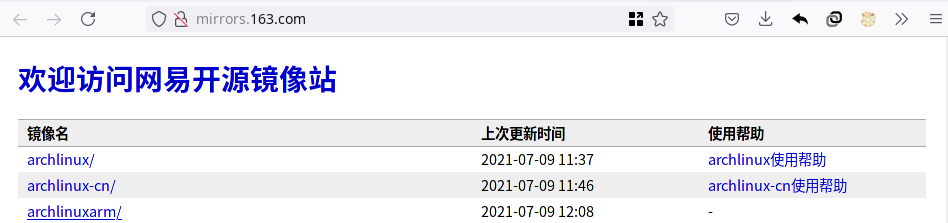
\includegraphics[width=0.8\textwidth]{fig/mirrors163com.png}
					\caption*{http://mirrors.163.com/}
				\end{figure}
			
				然后找到 \texttt{ubuntu-releases}。
				
				\begin{figure}[H]
					\centering
					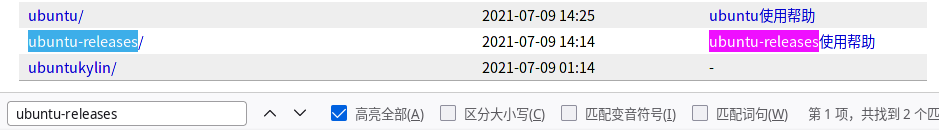
\includegraphics[width=0.8\textwidth]{fig/mirrors163com_find.png}
					\caption*{找到 ubuntu-releases}
				\end{figure}
				
				然后选择正确的版本。
				
				\begin{figure}[H]
					\centering
					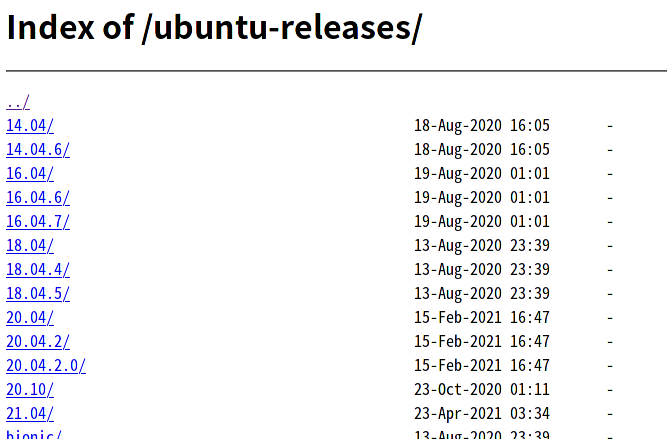
\includegraphics[width=0.8\textwidth]{fig/mirrors163com_in_ubuntu-releases.png}
					\caption*{/ubuntu-releases/}
				\end{figure}
			
				下载桌面版,即名字里面有 desktop 的那个。
				
				\begin{figure}[H]
					\centering
					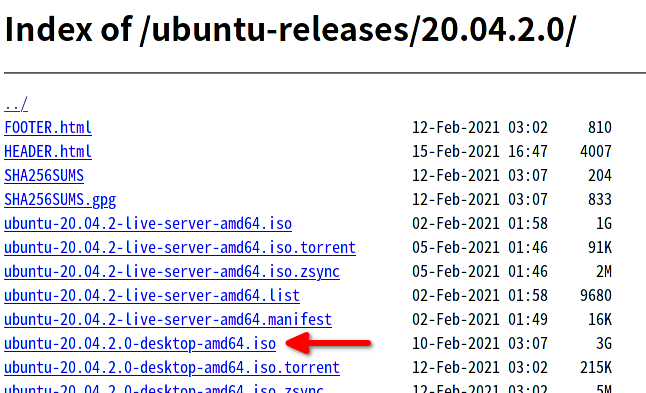
\includegraphics[width=0.8\textwidth]{fig/mirrors163com_choose_ubuntu-releases.png}
					\caption*{选择桌面版}
				\end{figure}
			
		\subsection{制作启动盘}
		
			\subsubsection{在 Linux 下}
			
				系统但凡是有点良心都会自带一个启动盘创建器。比如笔者的:
			
				\begin{figure}[H]
					\centering
					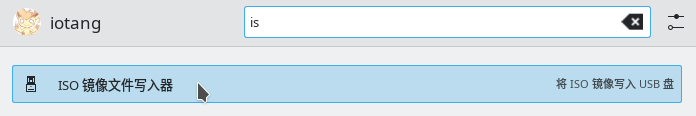
\includegraphics[width=0.8\textwidth]{fig/iso_burn.png}
					\caption*{KDE 下的启动盘创建器}
				\end{figure}
				
				此时,你需要准备一个 U 盘(最好至少 8 GB,并且笔者建议这个 U 盘应该是空的,以确保\textbf{\large 没有重要文件在里面}被抹去,因为制作启动盘时 U 盘里面的\textbf{\large 所有内容都会丢失}。)
				
				启动盘创建器的用法基本都一样。注意不要选错 U 盘。
			
				\begin{figure}[H]
					\centering
					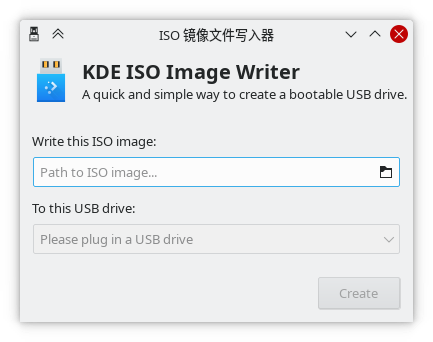
\includegraphics[width=0.3\textwidth]{fig/isoimagewriter.png}
					\caption*{KDE 启动盘创建器}
				\end{figure}


			\subsubsection{在 Windows 下}
			
				去下载 Rufus 启动盘创建器。
				
				\begin{figure}[H]
					\centering
					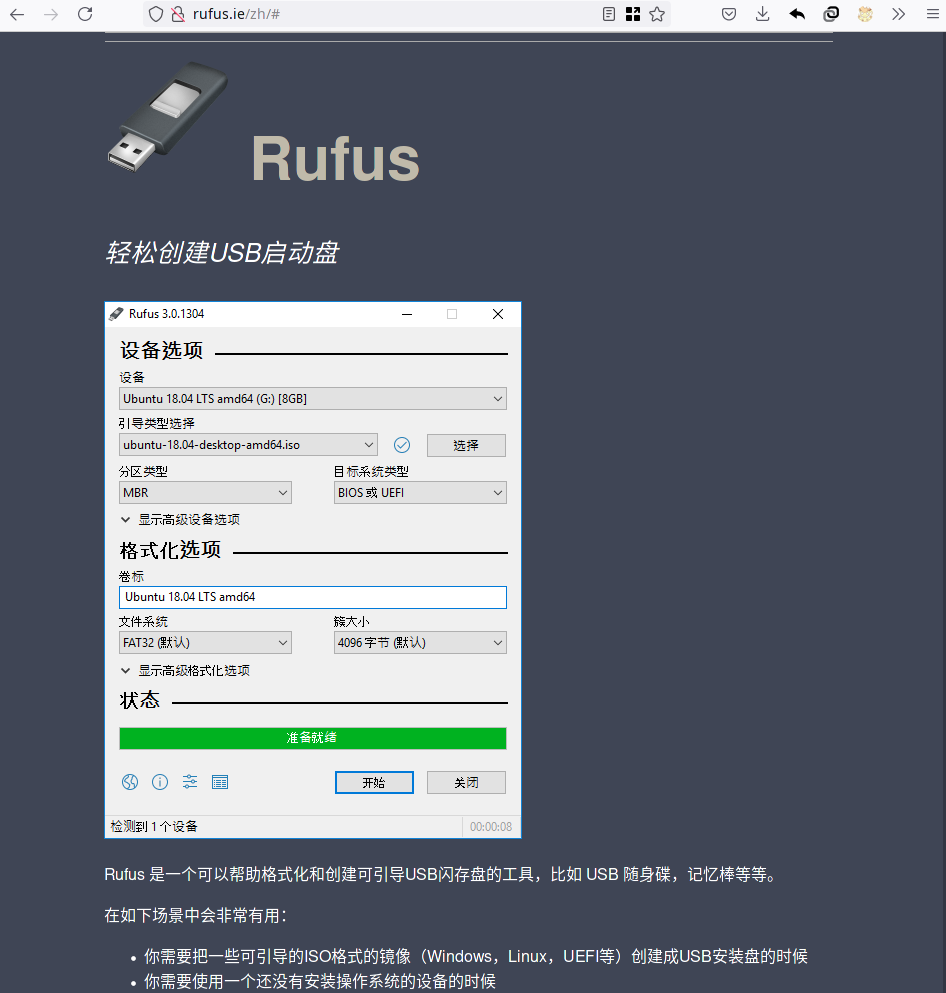
\includegraphics[width=0.8\textwidth]{fig/rufus.png}
					\caption*{Rufus}
				\end{figure}
			
		\subsection{安装 Ubuntu}
		
			我们马上会在目标电脑(机房里面的一台)上安装 Ubuntu。
		
			\subsubsection{BIOS 设置}
			
				首先打开目标电脑,从屏幕亮起来(甚至从电源键按下前)开始狂按 BIOS 键(比如 \texttt{F12}、\texttt{ESC}、\texttt{DEL} 等等)。
				
				在 BIOS 设置中打开 U 盘启动,打开 UEFI 模式优先(原先一般是 Legacy 优先)。
			
			\subsubsection{开始安装}
				
				关机,插上启动盘,开机时仍然狂按 BIOS 键,之后会出来一个界面让你选择启动位置。选择你的 U 盘(一般叫 USB-HDD 什么的)。
				
				之后在试用 Ubuntu 和安装 Ubuntu 中选择安装 Ubuntu。
				
				\begin{figure}[H]
					\centering
					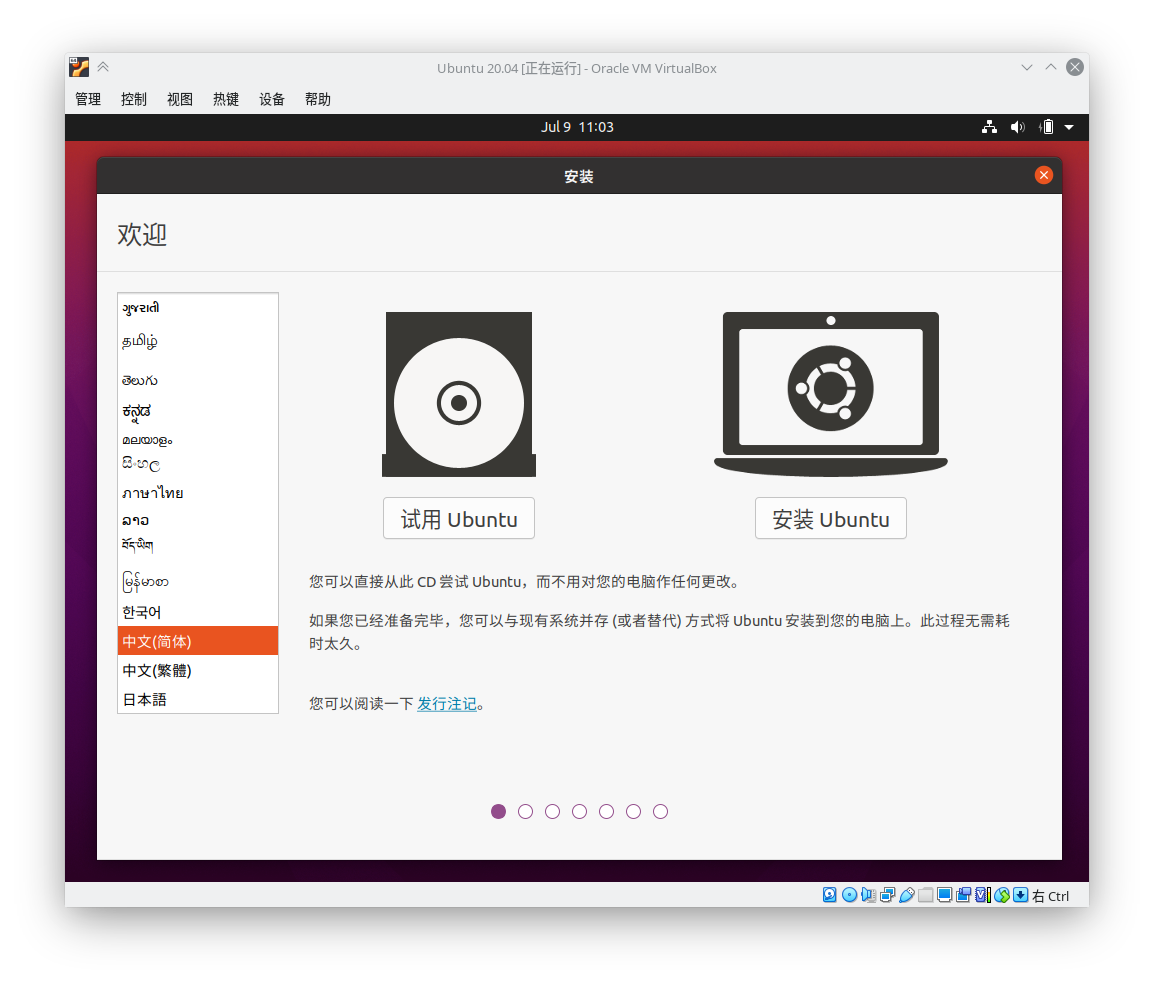
\includegraphics[width=0.7\textwidth]{fig/ubuntu_install_1.png}
					\caption*{安装 Ubuntu}
				\end{figure}
			
				选择键盘布局为 English (US)。
			
				\begin{figure}[H]
					\centering
					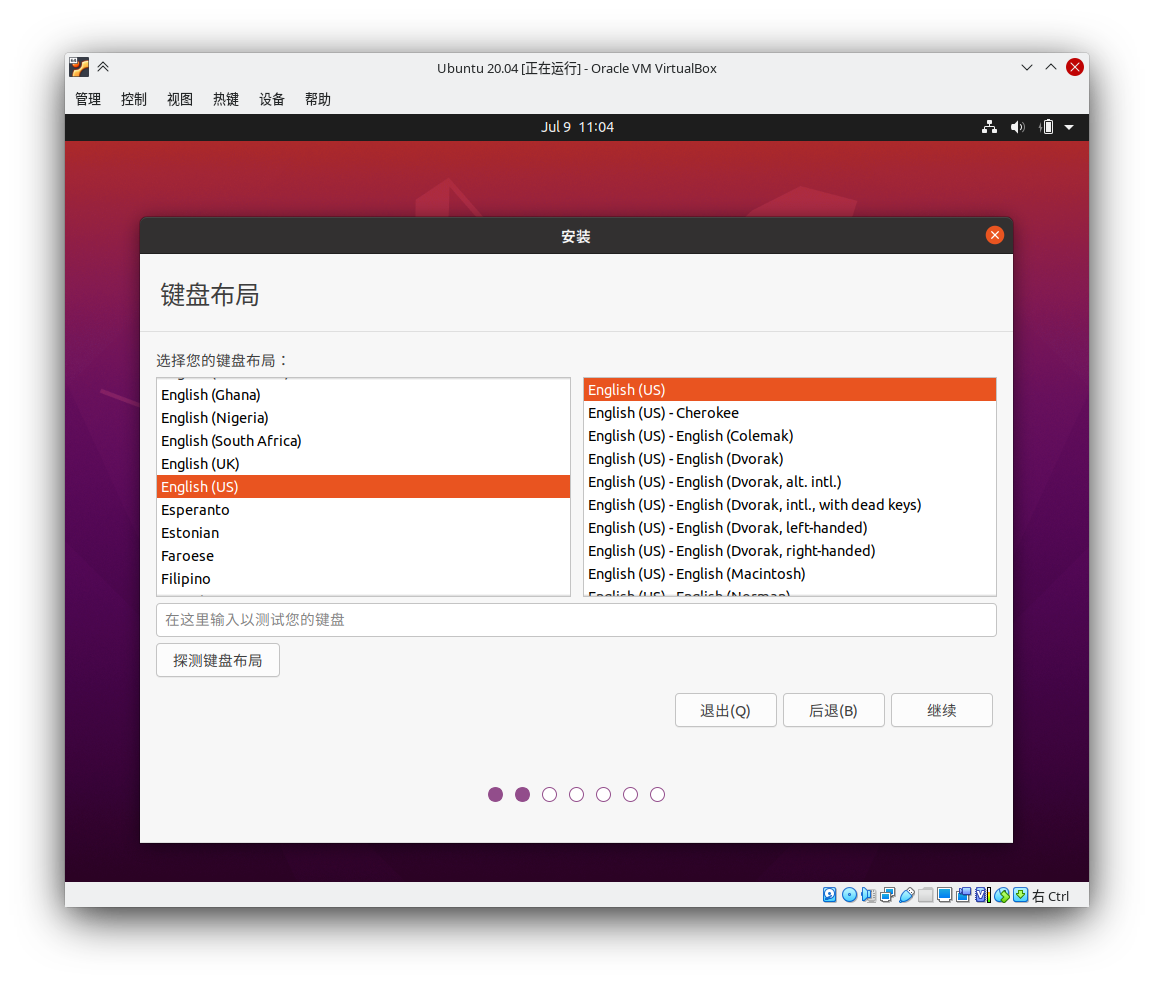
\includegraphics[width=0.7\textwidth]{fig/ubuntu_install_2.png}
					\caption*{选择键盘布局}
				\end{figure}
			
				建议先选择“最小安装”,并且不选“安装 Ubuntu 时下载更新”。
			
				\begin{figure}[H]
					\centering
					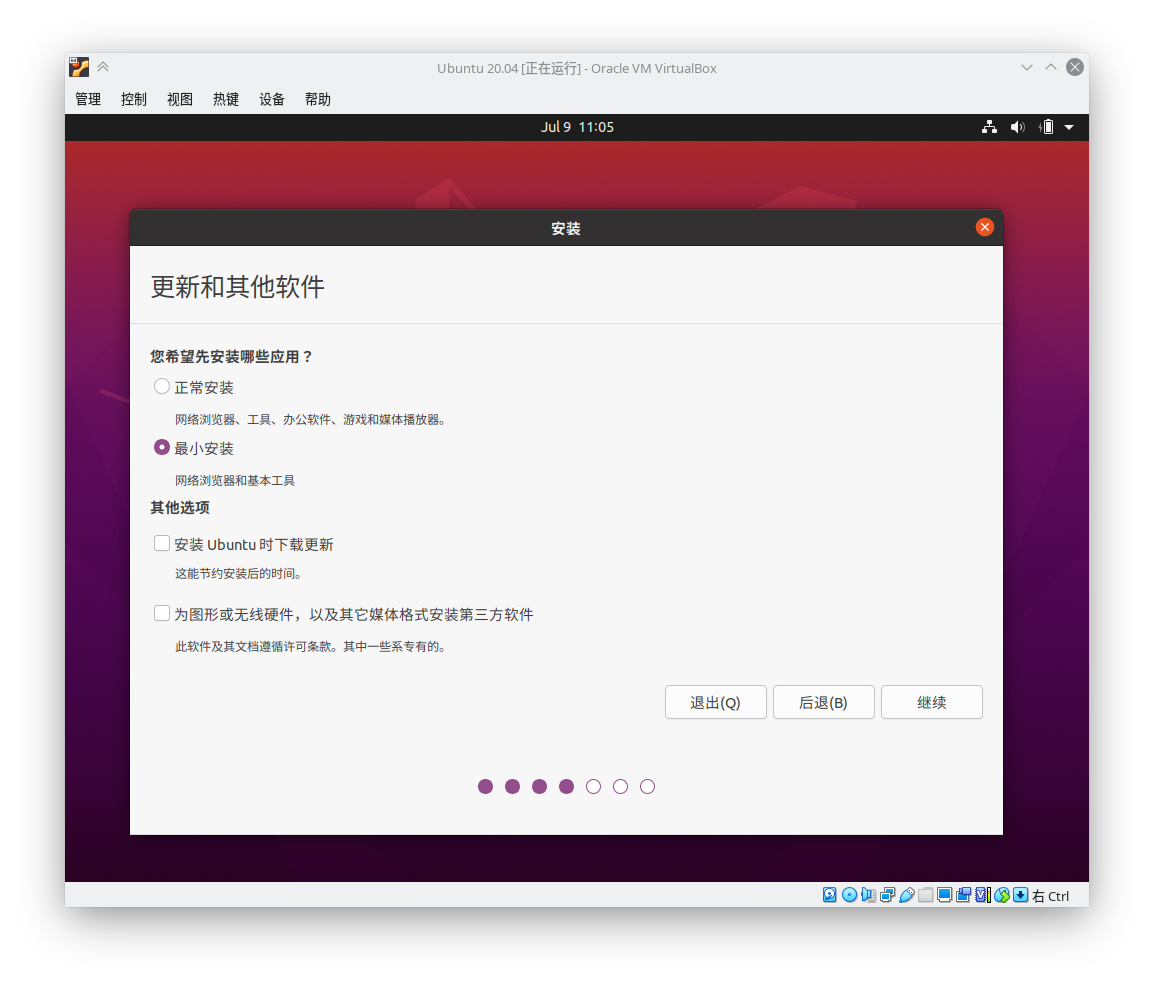
\includegraphics[width=0.7\textwidth]{fig/ubuntu_install_4.png}
					\caption*{更新和其他软件}
				\end{figure}
			
				根据需要选择安装类型。
			
				\begin{figure}[H]
					\centering
					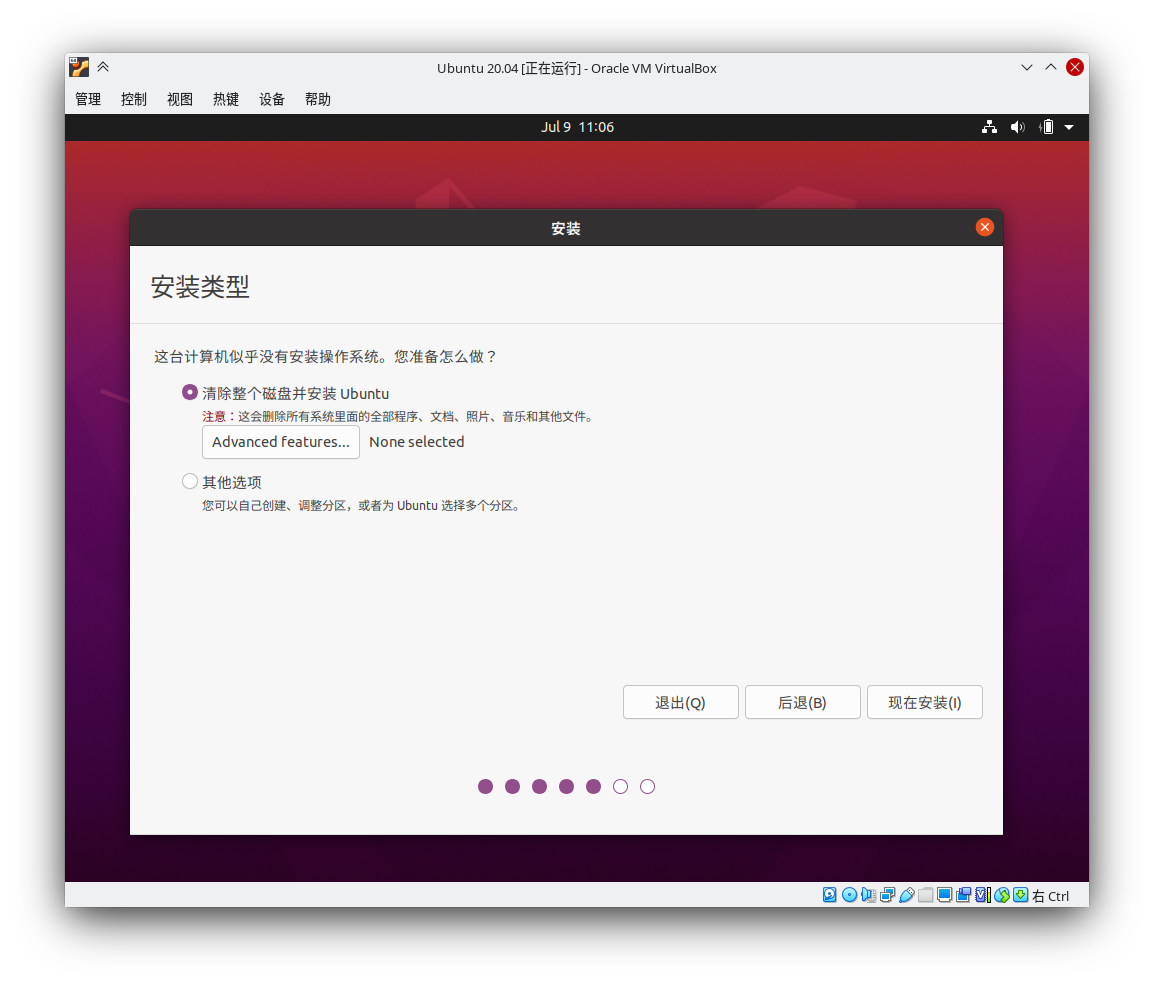
\includegraphics[width=0.7\textwidth]{fig/ubuntu_install_5.png}
					\caption*{安装类型}
				\end{figure}
			
				选择时区。
			
				\begin{figure}[H]
					\centering
					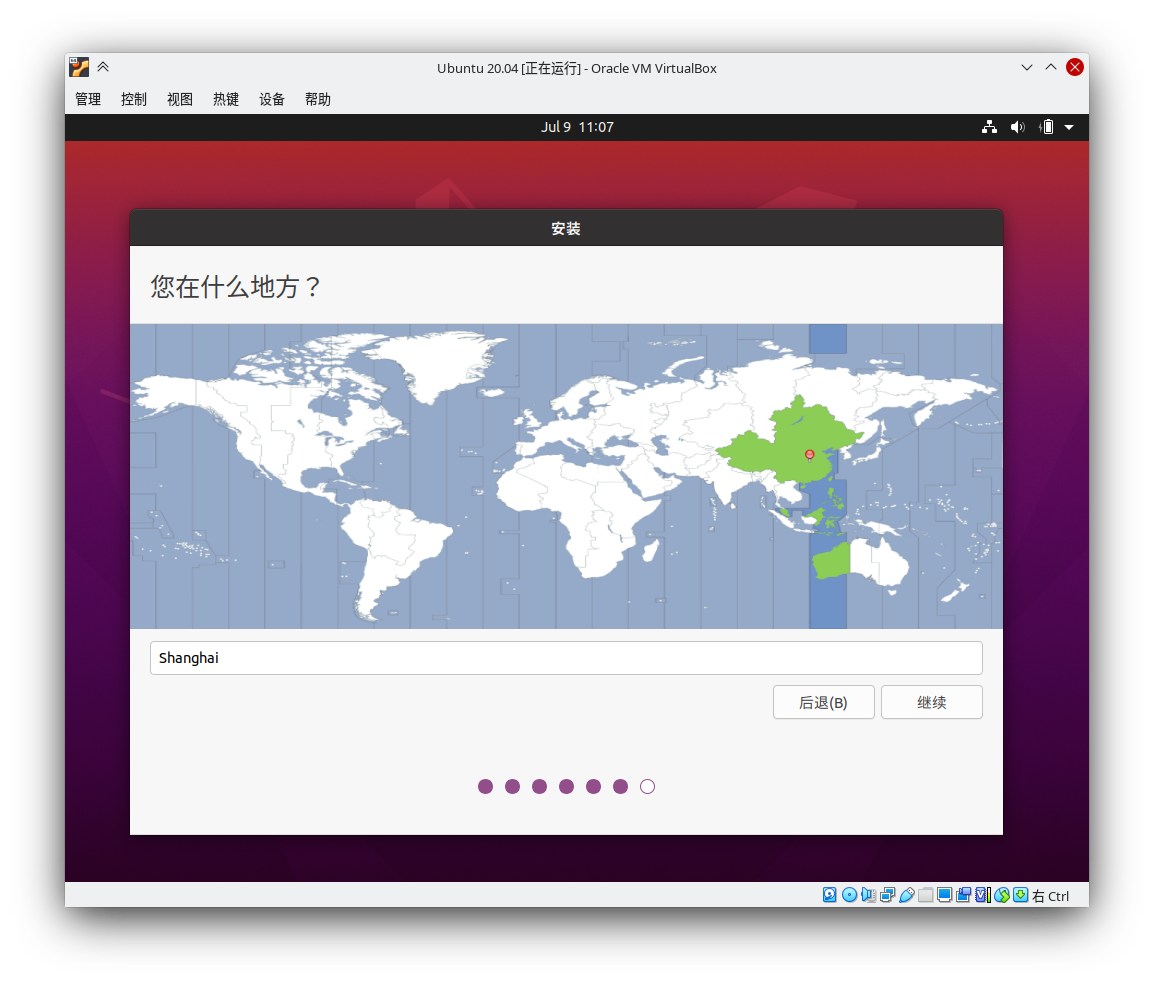
\includegraphics[width=0.7\textwidth]{fig/ubuntu_install_6.png}
					\caption*{我是中国弗兰常杀人}
				\end{figure}
			
				设置第一个用户。
				
				\begin{figure}[H]
					\centering
					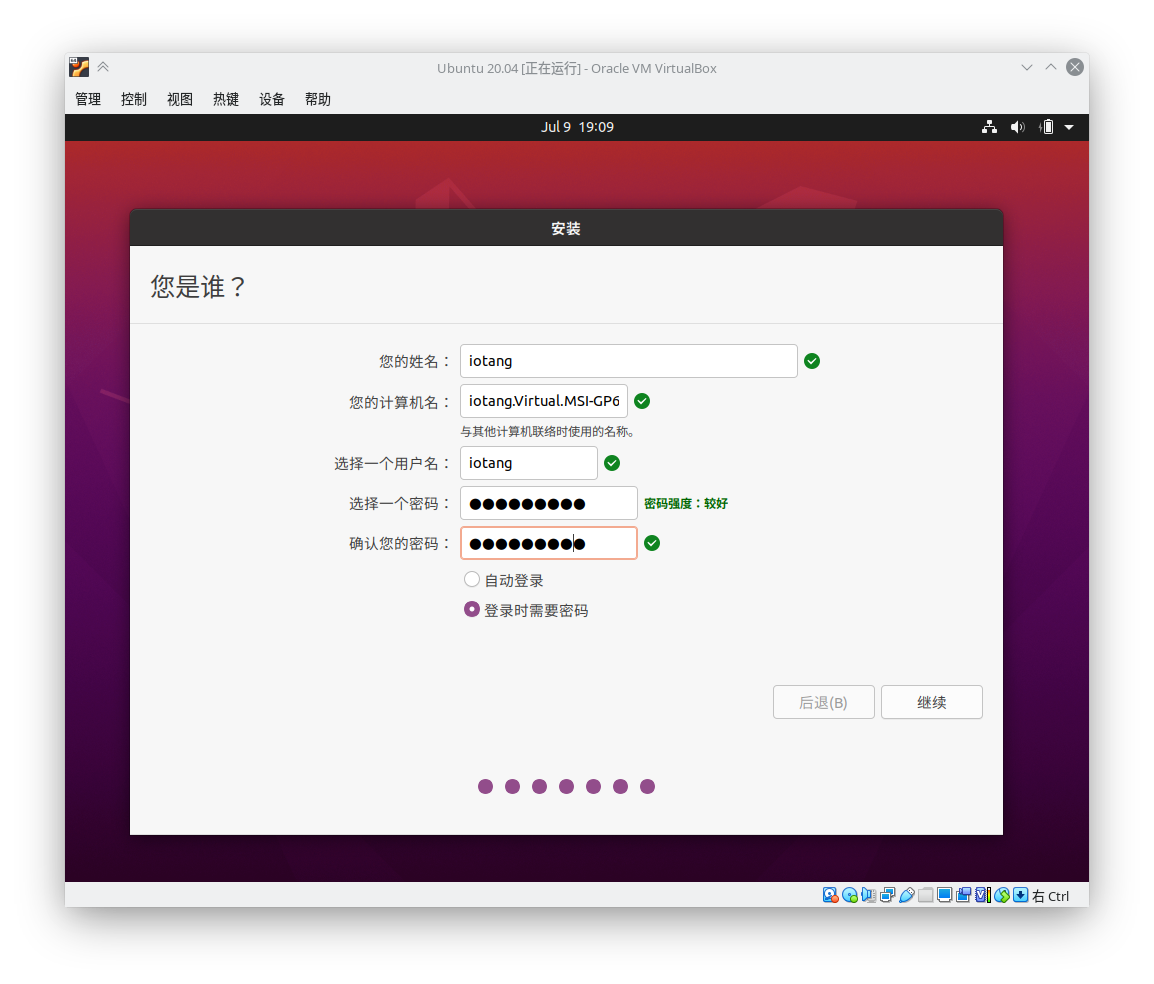
\includegraphics[width=0.7\textwidth]{fig/ubuntu_install_7.png}
					\caption*{第一个用户一定是管理员}
				\end{figure}
			
				建议把网络关掉,以防安装程序用巨慢的速度下载一些东西,把安装时间拖得很长。
			
				\begin{figure}[H]
					\centering
					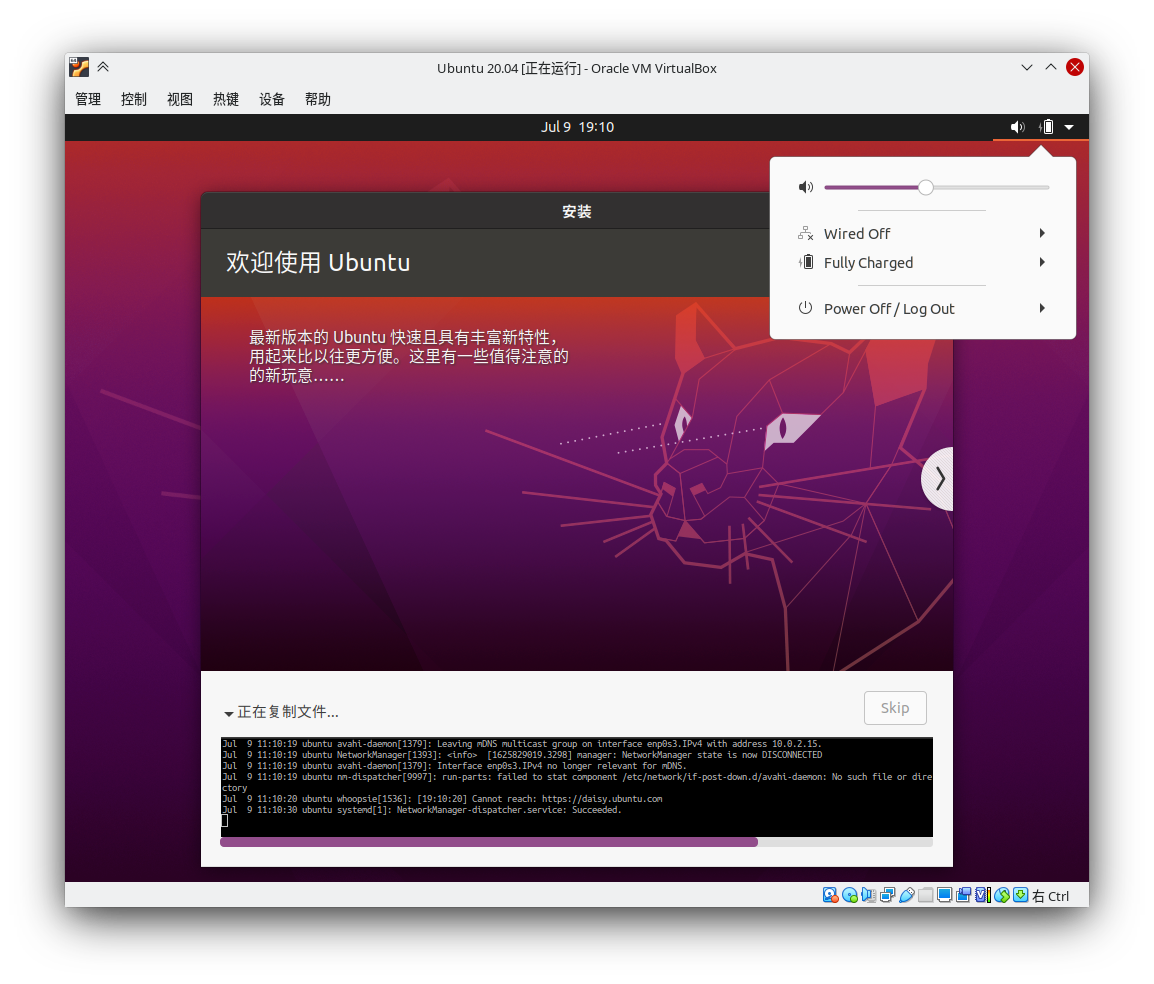
\includegraphics[width=0.7\textwidth]{fig/ubuntu_install_8.png}
					\caption*{关闭网络}
				\end{figure}
			
				之后关机,然后拔掉启动盘后开机。
				
				准备迎接 Ubuntu!第一次启动可能非常慢。
				
				在上图中你可以看到一只哺乳动物。这是 Focal Fossa,Ubuntu 20.04 的吉祥物。“Fossa”是马达加斯加长尾灵猫。
			
	\newpage
		
	\section{初始设置}
	
		\subsection{终端命令的使用}
		
			无论如何,你必须得学会终端的使用方式。
		
			用快捷键 \texttt{Ctrl + Alt + T} 打开一个终端。
			
			\begin{figure}[H]
				\centering
				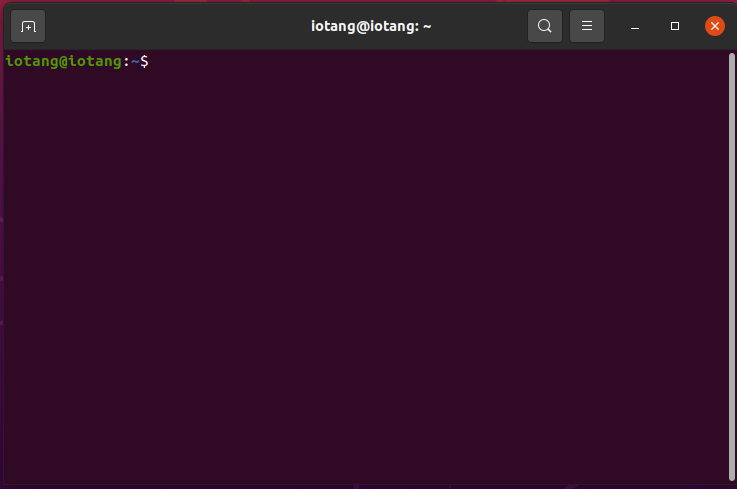
\includegraphics[width=0.8\textwidth]{fig/terminal.png}
				\caption*{一个终端}
			\end{figure}
		
			在“\texttt{\$}”前面的内容是这样:
			
			\texttt{\huge {\color{red}用户名}{\color{brown}@}{\color{olive}主机名}{\color{cyan}:}{\color{blue}当前目录}\$}
			
			\texttt{\huge {\color{red}iotang}{\color{brown}@}{\color{olive}iotang}{\color{cyan}:}{\color{blue}\textasciitilde}\$}
		
			\subsubsection{基本快捷键}
			
				\texttt{Tab 键} ~自动补全。
				
				\texttt{Ctrl + c} 中断当前正在运行的程序。
				
				\texttt{Ctrl + Shift + c} 复制。
				
				\texttt{Ctrl + Shift + v} 粘贴。
			
			\subsubsection{基本命令}
			
				\texttt{sudo} 以管理员权限运行之后的命令,即 \textbf{S}uper \textbf{U}ser \textbf{Do}。
				
				\texttt{man} 查询手册。比如查询命令 \texttt{sudo}:输入\texttt{man sudo}。请通过自己的能力找到以下命令的详细用法,并自己练习。
			
			\subsubsection{对于文件和目录的命令}
			
				\texttt{\textasciitilde} 家目录,即 \texttt{/home/你的用户名}。默认打开终端进入的就是你的家目录。
				
				\texttt{.} 现在的目录。
				
				\texttt{..} 上一级目录。
				
				\texttt{pwd} 显示当前位置,即 print working directory。
				
				\texttt{ls} 列出当前目录下的文件与目录,即 list。
				
				\texttt{ls -l} 列出当前目录下的文件与目录,显示文件相关属性。
				
				\texttt{ls -a} 列出当前目录下的文件与目录,包括隐藏文件。
				
				\texttt{ls -la} 列出当前目录下的文件与目录(包括隐藏文件),并显示文件相关属性。
				
				\texttt{cd} 改变目录,即 change directory。
				
				\texttt{cd ..} 进入上一级目录。
				
				\texttt{cp} 复制,即 copy。
				
				\texttt{mv} 移动,即 move。
				
				\texttt{rm} 删除,即 remove。不可撤销!
				
				\texttt{mkdir} 创建目录,即 make directory。
				
				\texttt{rmdir} 删除目录。
				
			\subsubsection{对于系统状态的命令}
			
				\texttt{df} 显示文件系统中还有多少剩余空间。
				
				\texttt{df -h} 显示文件系统中还有多少剩余空间,用兆字节和吉字节为单位来显示设备空间使用量。\texttt{-h} 的 h 是 human-readable 的意思,因为默认是用千字节为单位来表示使用量的。
				
				\texttt{free} 显示内存使用情况。
				
				\texttt{free -m} 以兆字节为单位显示内存使用情况。
				
				\texttt{uname -a} 显示所有的系统信息。
				
				\texttt{lsb\_release -a} 显示当前 Ubuntu 版本。
				
				
	
		\subsection{第一次更新软件}
		
			\subsubsection{更换软件源}
		
				更换 Ubuntu 的软件源到国内某一个,否则软件安装和更新的速度将非常慢,因为默认源地址不在国内。
				
				这边以清华大学开源软件镜像站为例子:
				
				百度到清华大学开源软件镜像站 Ubuntu 镜像使用帮助。
					
				\begin{figure}[H]
					\centering
					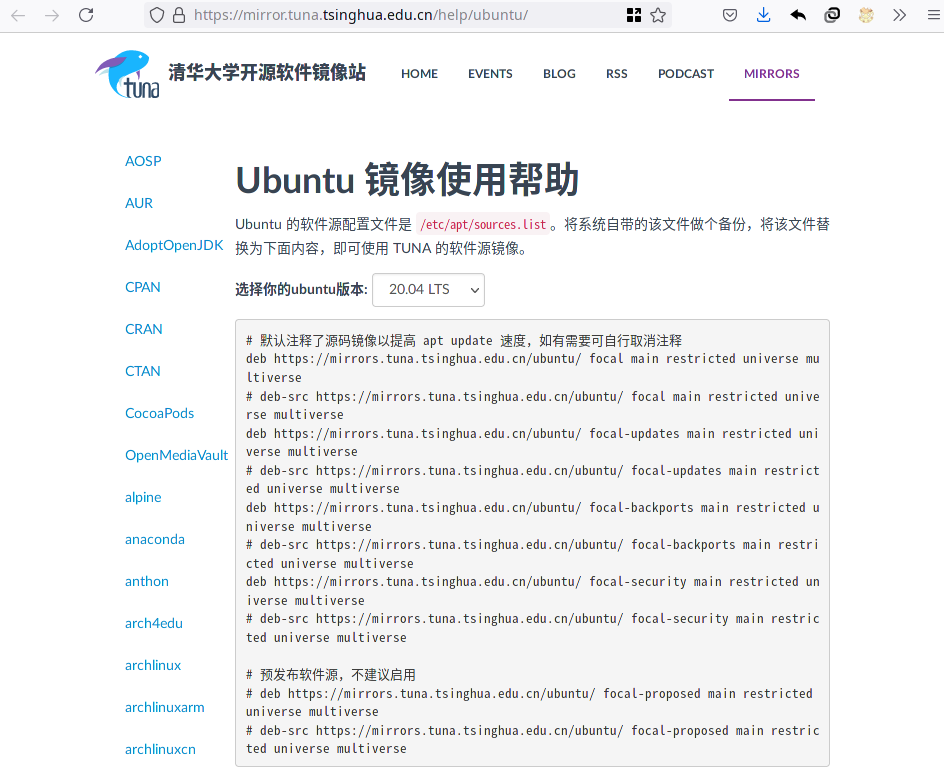
\includegraphics[width=0.8\textwidth]{fig/ubuntu_mirror_help.png}
					\caption*{贵校镜像站 Ubuntu 镜像使用帮助}
				\end{figure}
			
				选择正确的 Ubuntu 版本,复制镜像内容,然后编辑 \texttt{/etc/apt/sources.list}:
	
				\begin{minted}[frame=single]{console}
$ sudo gedit /etc/apt/sources.list
				\end{minted}
			
				\texttt{gedit} 是 GNOME 桌面下的一个文本编辑器,即 \textbf{G}nome \textbf{Edit}。
				
				从这里开始,以“\texttt{\$}”开头的东西代表你要在终端中执行这个语句(执行的语句里面没有“\texttt{\$}”)。比如对于上面那个命令,你可以先用快捷键 \texttt{Ctrl + Alt + T} 打开一个终端,然后输入 \texttt{sudo gedit /etc/apt/sources.list}(没有 “\texttt{\$}”):
	
				\begin{figure}[H]
					\centering
					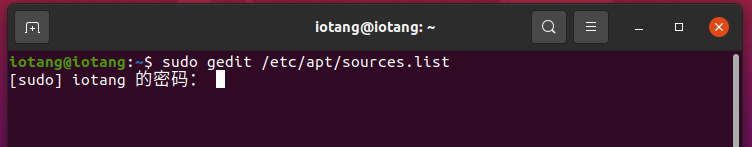
\includegraphics[width=0.8\textwidth]{fig/gedit_etcaptsourceslist.png}
					\caption*{打开 /etc/apt/sources.list}
				\end{figure}
				
				用你找到的镜像内容替换文件里原来的所有内容。
				
				\begin{figure}[H]
					\centering
					\begin{minipage}{0.41\textwidth}
						\centering
						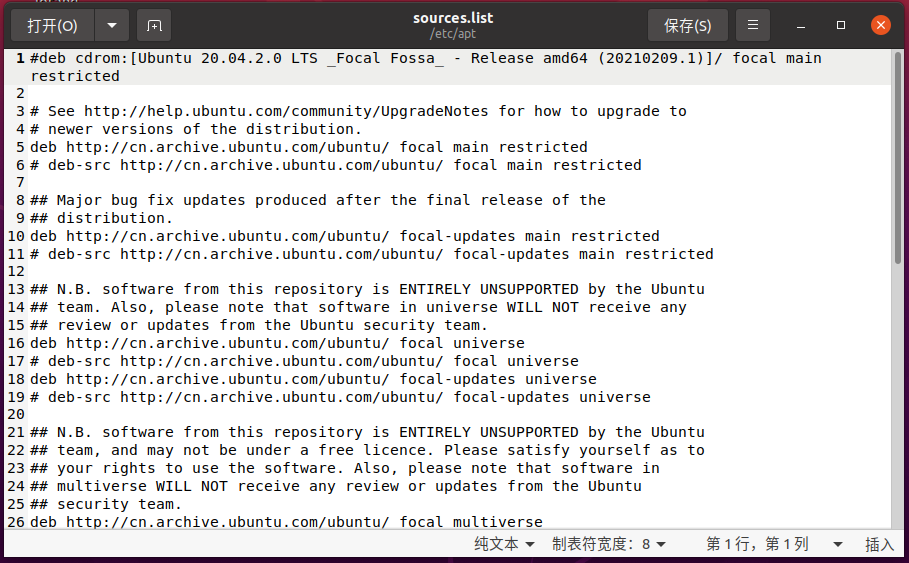
\includegraphics[width=\textwidth]{fig/sourceslist_before.png}
						\caption*{替换前}
					\end{minipage}
					\begin{minipage}{0.41\textwidth}
						\centering
						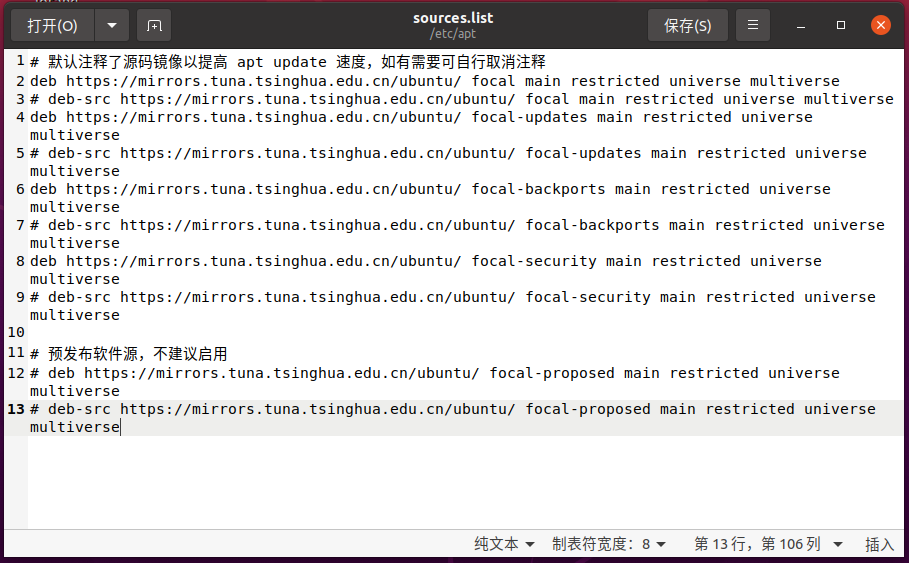
\includegraphics[width=\textwidth]{fig/sourceslist_after.png}
						\caption*{替换后}
					\end{minipage}
				\end{figure}
			
			\subsubsection{apt 是什么?}
			
				注意到了上文的 \texttt{/etc/apt/sources.list} 中的 apt 了吗?
	
				apt 是 Linux 下的安装包管理工具之一。Ubuntu 使用 apt。
				
			\subsubsection{更新软件列表}
				
				\begin{minted}[frame=single]{console}
$ sudo apt update
				\end{minted}
			
				更新软件列表可以让 apt 知道现在有哪些软件,以及那些软件的版本。
				
				apt 会将软件列表和目前的状况比对,然后就可以得出哪些软件可以更新。
				
				\begin{figure}[H]
					\centering
					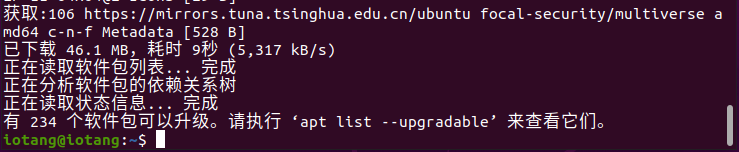
\includegraphics[width=0.8\textwidth]{fig/apt_update.png}
					\caption*{apt 找到了好多可以更新的软件}
				\end{figure}
			
			\subsubsection{更新软件}
	
				\begin{minted}[frame=single]{console}
$ sudo apt upgrade
				\end{minted}
				
				这可以让 apt 更新目前所有的软件。
				
				\begin{figure}[H]
					\centering
					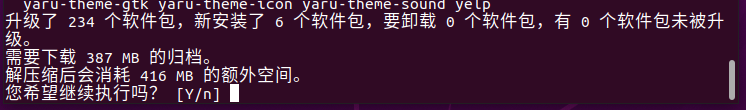
\includegraphics[width=0.8\textwidth]{fig/apt_upgrade_yn.png}
					\caption*{确定界面}
				\end{figure}
			
				在这里,\texttt{[Y/n]} 的 \texttt{Y} 是大写,意味着默认是“是”。也就是说,如果你在这里直接按下回车,那么就按“是”处理。
				
			\subsubsection{查找软件}
				
				\begin{minted}[frame=single]{console}
$ apt search xxx
				\end{minted}
			
				让 apt 在软件列表里查找相应字段。比如我想安装一个文本编辑软件 Emacs:
				
				\begin{minted}[frame=single]{console}
$ apt search emacs
				\end{minted}
			
				可以发现有一个软件包叫 emacs。
				
				\begin{figure}[H]
					\centering
					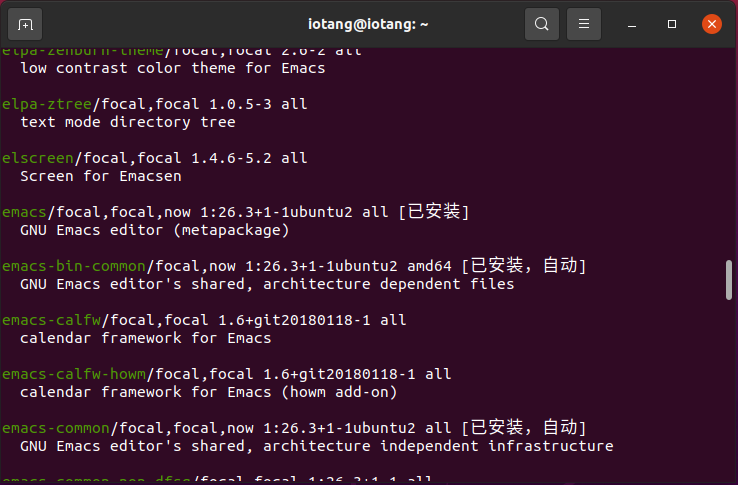
\includegraphics[width=0.8\textwidth]{fig/apt_find_emacs.png}
					\caption*{apt 找到了 Emacs}
				\end{figure}

			\subsubsection{安装软件}
		
				\begin{minted}[frame=single]{console}
$ sudo apt install xxx
				\end{minted}
				
				比如我们刚才找到了 Emacs 的软件名就叫 emacs,所以我们可以这样安装 emacs:
				
				\begin{minted}[frame=single]{console}
$ sudo apt install emacs
				\end{minted}
			
		\subsection{安装中文输入法}
		
			Linux 下想输入中文的话,一个方法是使用输入法。而搜狗输入法在 Linux 下仍然可用。
			
			百度到给 Linux 的搜狗输入法的主页:
		
			\begin{figure}[H]
				\centering
				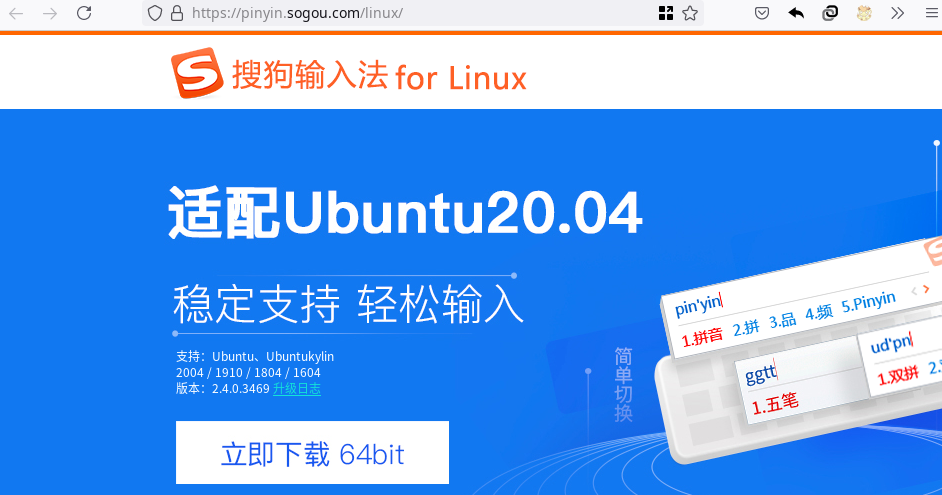
\includegraphics[width=0.8\textwidth]{fig/sogou.png}
				\caption*{搜狗输入法已经支持到了 Ubuntu 20.04}
			\end{figure}
	
			下载会得到一个以 \texttt{.deb} 结尾的安装包:\texttt{sogoupinyin\_版本号\_amd64.deb}。
			
			\begin{figure}[H]
				\centering
				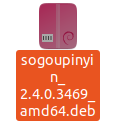
\includegraphics[width=0.2\textwidth]{fig/sogoupinyin_deb.png}
				\caption*{搜狗拼音安装包}
			\end{figure}
			
			\subsubsection{添加中文语言支持}
			
				打开系统设置,找到“区域和语言”,点击“管理已安装的语言”。
				
				\begin{figure}[H]
					\centering
					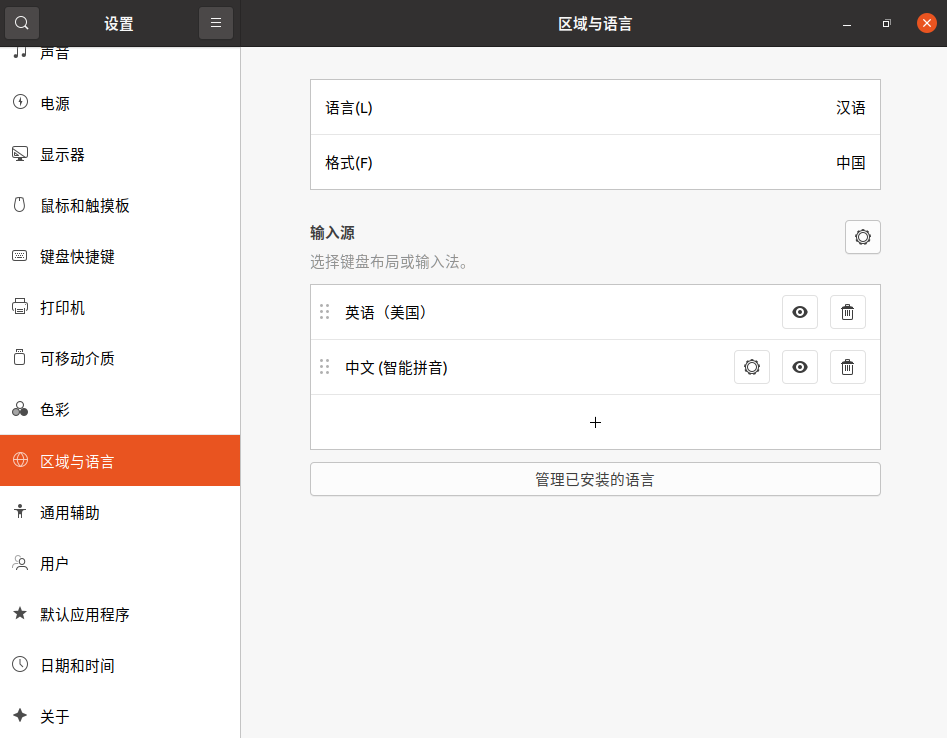
\includegraphics[width=0.8\textwidth]{fig/settings_locs_and_langs.png}
					\caption*{区域和语言}
				\end{figure}
			
				如果有语言支持没有安装完整,可以选择安装。
				
				\begin{figure}[H]
					\centering
					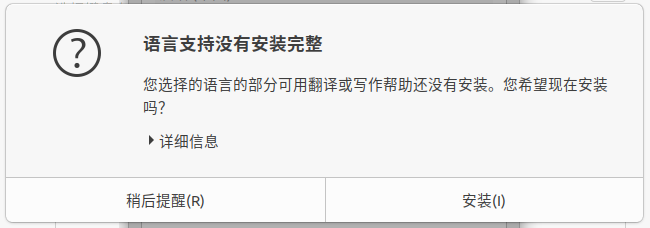
\includegraphics[width=0.8\textwidth]{fig/langs_support.png}
					\caption*{语言支持没有安装完整}
				\end{figure}
				
				在“语言”栏下点击“添加或删除语言”。
				
				\begin{figure}[H]
					\centering
					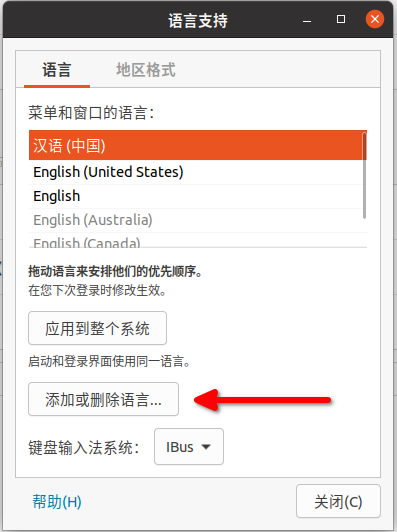
\includegraphics[width=0.4\textwidth]{fig/add_or_del_langs.png}
					\caption*{添加或删除语言}
				\end{figure}
				
				在弹出来的窗口里勾上“中文(简体)”,应用。
				
				\begin{figure}[H]
					\centering
					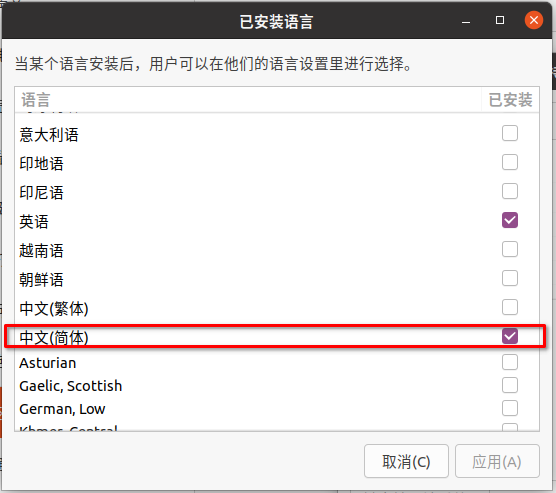
\includegraphics[width=0.6\textwidth]{fig/add_zh_cn.png}
					\caption*{添加中文(简体)}
				\end{figure}
			
			\subsubsection{切换到 fcitx}
	
				回到“语言支持”窗口,在键盘输入法系统中,选择“fcitx”。
				
				\begin{figure}[H]
					\centering
					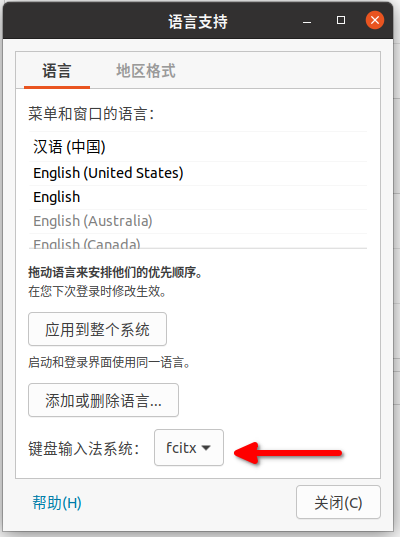
\includegraphics[width=0.4\textwidth]{fig/choose_fcitx.png}
					\caption*{选择 fcitx}
				\end{figure}
				
				如果没有 fcitx,那么把 fcitx 装上:
				
				\begin{minted}[frame=single]{console}
$ sudo apt install fcitx
				\end{minted}
			
				选择“应用到整个系统”。
				
				\begin{figure}[H]
					\centering
					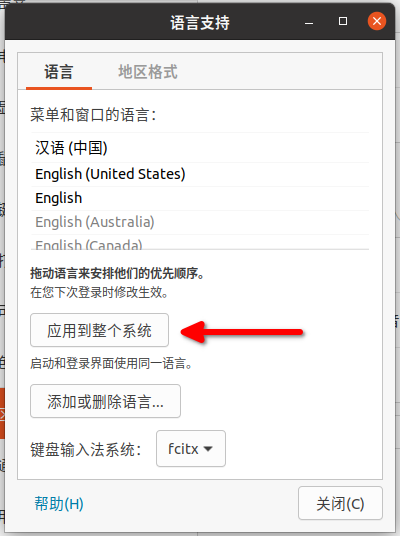
\includegraphics[width=0.4\textwidth]{fig/apply_langs_settings.png}
					\caption*{应用到整个系统}
				\end{figure}
			
			\subsubsection{安装搜狗输入法}
			
				直接双击打开这个安装包,在弹出的应用商店里安装。
			
				\begin{figure}[H]
					\centering
					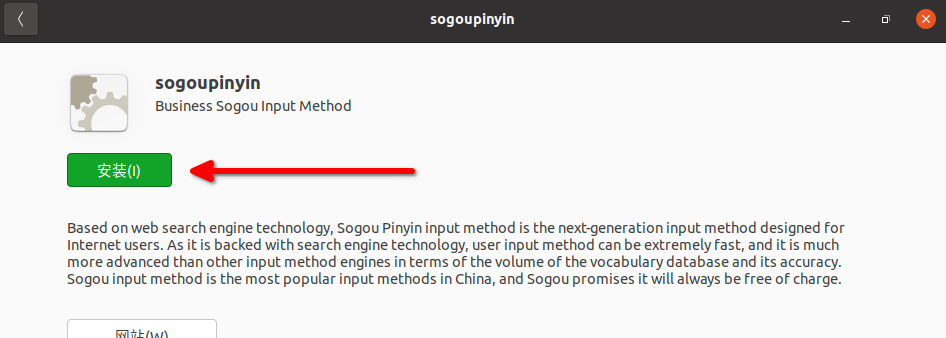
\includegraphics[width=0.8\textwidth]{fig/sogoupinyin_install.png}
					\caption*{安装搜狗拼音}
				\end{figure}
			
				重启系统,发现搜狗输入法已经在列表中。
				
				\begin{figure}[H]
					\centering
					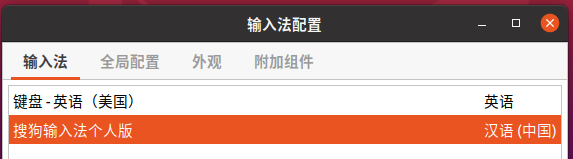
\includegraphics[width=0.8\textwidth]{fig/add_sogou_success.png}
					\caption*{搜狗拼音已经可以使用}
				\end{figure}
			
				用 \texttt{Ctrl + Space} 切换输入法,就可以使用搜狗输入法了。
				
				\begin{figure}[H]
					\centering
					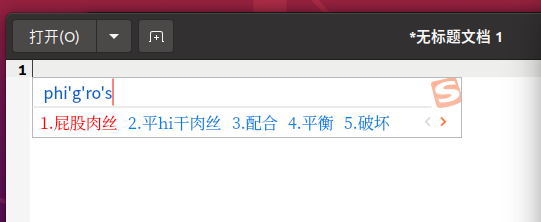
\includegraphics[width=0.8\textwidth]{fig/sogou_success.png}
					\caption*{大~功~告~成}
				\end{figure}
				
	\newpage
				
	\section{完善工作环境}
	
		\subsection{在右键菜单中添加“新建文件”}
		
			\begin{minted}[frame=single]{console}
$ cd ~/Templates
$ touch "空白文档.txt"
			\end{minted}
		
			\textbf{想一想:}上面的两行命令分别有什么作用?
			
			\textbf{练习:}让右键菜单“新建文件”中出现一个“新建 C++ 文件”。
	
		\subsection{以 Emacs 作为 C++ 代码编辑器}
		
			这里我假设大家都是 C++ 选手。
			
			Emacs 是著名的集成开发环境和文本编辑器,被公认为是最受专业程序员喜爱的代码编辑器之一。
			
			你可以在任何地方看见 Emacs 教徒和 Vim 教徒之间的争端。
			
			而 Emacs 比较符合正常人的操作逻辑,所以我们暂且把 Vim 放到一边,来使用 Emacs。
		
			\subsubsection{安装}
		
				\begin{minted}[frame=single]{console}
$ sudo apt install emacs
				\end{minted}
			
			\subsubsection{配置 Emacs}
			
				首先搞到豪华配置:\href{https://www.luogu.com.cn/paste/uzsz2zf4}{网址}。
				
				\begin{figure}[H]
					\centering
					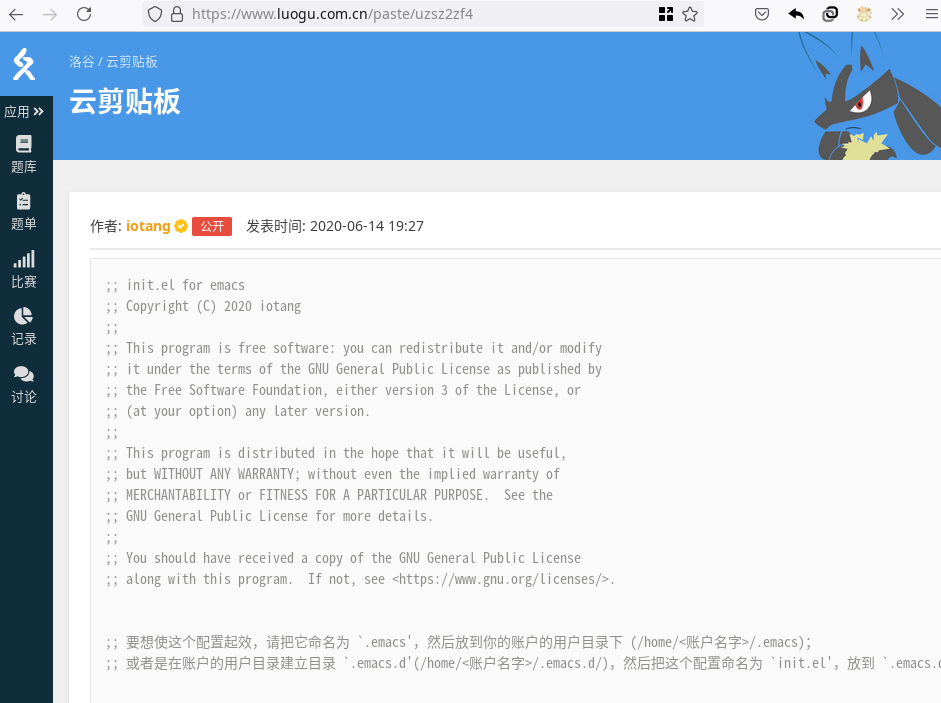
\includegraphics[width=0.8\textwidth]{fig/emacs_init_el.png}
					\caption*{当年 HNOI 省选赛场上的配置}
				\end{figure}
			
				要想使这个配置起效,请把它命名为 \texttt{.emacs},然后放到你的账户的用户目录下(\texttt{/home/<账户名字>/.emacs});
				
				\textbf{或者是}在账户的用户目录建立目录 \texttt{.emacs.d}(\texttt{/home/<账户名字>/.emacs.d/}),然后把这个配置命名为 \texttt{init.el},放到 \texttt{.emacs.d} 下。
				
				\begin{figure}[H]
					\centering
					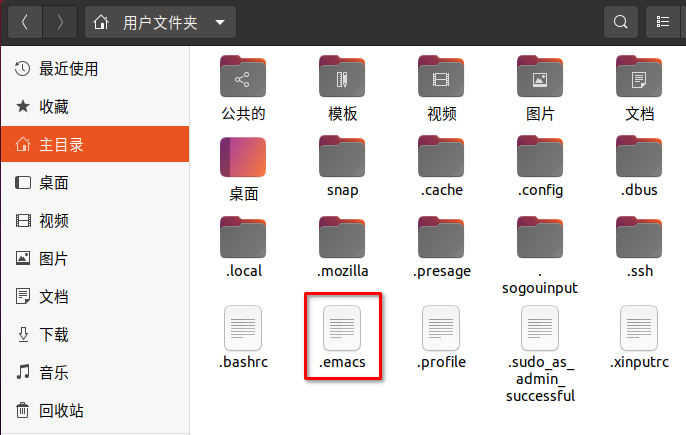
\includegraphics[width=0.8\textwidth]{fig/place_emacs.png}
					\caption*{.emacs}
				\end{figure}
			
				\begin{figure}[H]
					\centering
					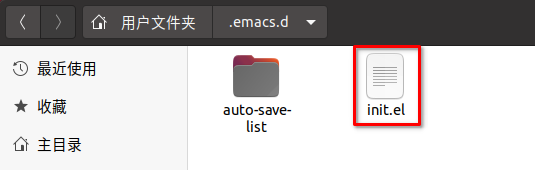
\includegraphics[width=0.8\textwidth]{fig/place_init_el.png}
					\caption*{.emacs.d/init.el}
				\end{figure}
				
				(以“\texttt{.}”开头的文件是隐藏文件。在文件管理器中按 \texttt{Ctrl + h} 显示它们。)
			
			\subsubsection{考场上在没有 Emacs 配置的时候配置 Emacs}
			
				之前提到的“配置”就是 Emacs 在启动之前会调用的一堆命令。
				
				Emacs 的命令的语言是 Emacs Lisp,语法基本都长这样:
				
				\begin{minted}[frame=single]{lisp}
(函数名字 参数 参数 参数 ...)
				\end{minted}
			
				半角分号“;”之后的内容都是注释:
				
				\begin{minted}[frame=single]{lisp}
(函数名字 参数 参数 参数 ...)     ;逮虾户
				\end{minted}
			
				比如:
				
				\begin{minted}[frame=single]{lisp}
(+ a b) ;; 加法
(- a b) ;; 减法
(defun 函数名 (参数表) 函数体) ;; 一个函数,效果是定义一个函数
				\end{minted}
			
				Lisp 尝试计算一切,包括函数的参数。单引号可以防止 Lisp 瞎计算东西:
				
				\begin{minted}[frame=single]{lisp}
(write (* 114 514)) ;; 输出 58596
(write '(* 114 514)) ;; 输出 (* 114 514)
				\end{minted}
				
				然后你可以在上面的配置中看到这个。
				
				\begin{minted}[frame=single]{lisp}
(defun compile-file ()(interactive)(compile 
(format "g++ %s -o %s -g -lm -Wall -std=c++98 -fsanitize=address" 
(buffer-name)(file-name-sans-extension (buffer-name)))))
				\end{minted}
			
				我们再加几个换行。
				
				\begin{minted}[frame=single]{lisp}
(defun compile-file ()(interactive)
    (compile 
        (format
            "g++ %s -o %s -g -lm -Wall -std=c++98 -fsanitize=address" 
            (buffer-name)(file-name-sans-extension (buffer-name))
        )
    )
)
				\end{minted}
			
				(interactive 表示它可以通过 \texttt{M-x} 调用。)
				
				呃,就是这样。
				
				然后没有配置的 Emacs 是这样的:
				
				\begin{figure}[H]
					\centering
					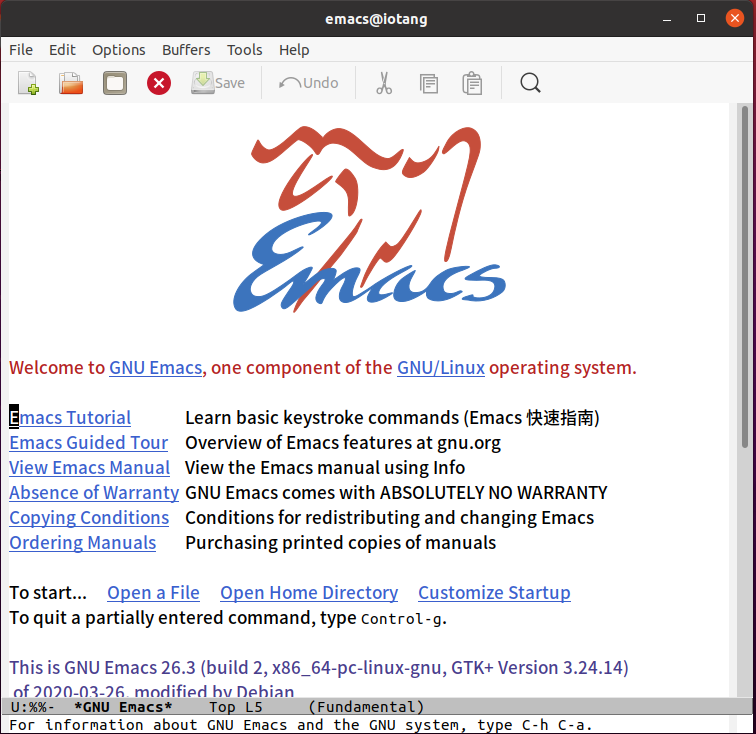
\includegraphics[width=0.6\textwidth]{fig/emacs_orig.png}
					\caption*{Emacs 原本的模样}
				\end{figure}
				
				首先通过非命令方法设置:
				
				在这里可以设置括号匹配和设置 CUA 键(剪切、复制、粘贴分别是 \texttt{C-x}, \texttt{C-c}, \texttt{C-v}(大写的 C 代表 \texttt{Ctrl},大写的 \texttt{M} 代表 \texttt{Alt})),以及\textbf{\large 保存设置}。
				
				\begin{figure}[H]
					\centering
					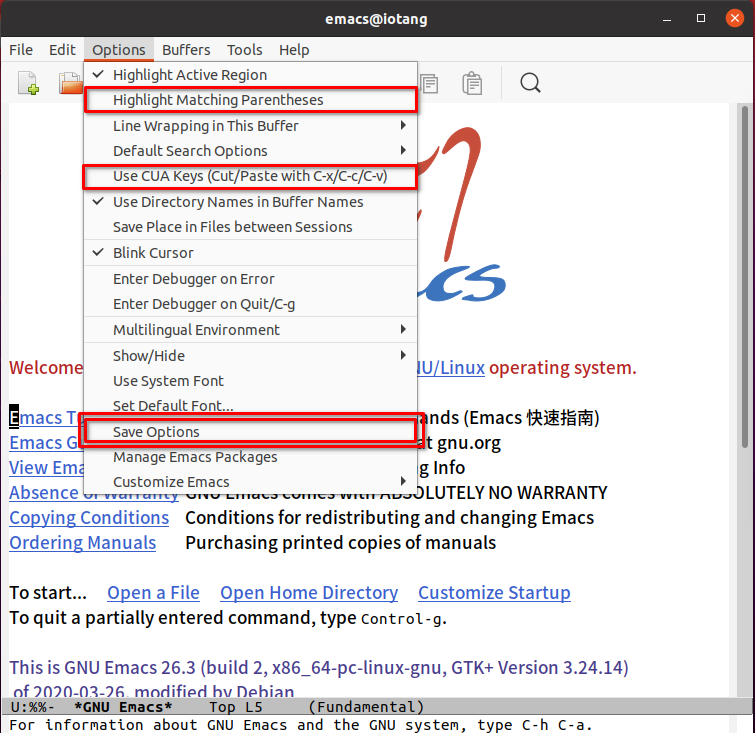
\includegraphics[width=0.6\textwidth]{fig/emacs_options.png}
					\caption*{Emacs 设置}
				\end{figure}
			
				在这里可以设置 Emacs 的各种东西是否显示。
				
				\begin{figure}[H]
					\centering
					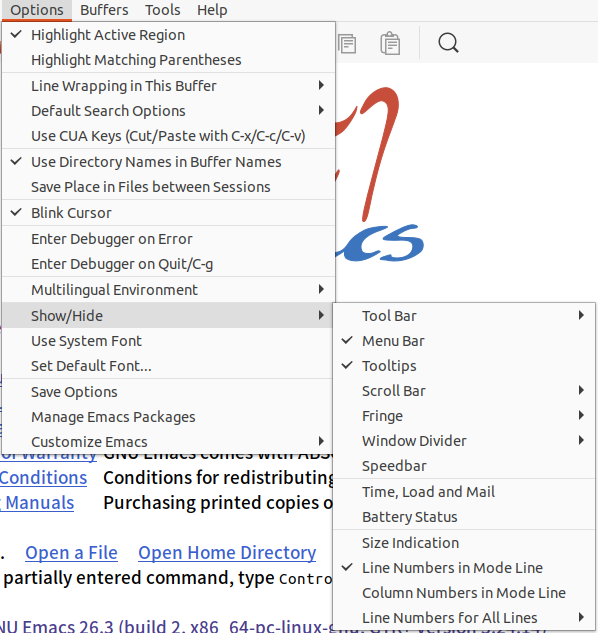
\includegraphics[width=0.6\textwidth]{fig/emacs_show_hide.png}
					\caption*{Emacs 设置显示 / 隐藏}
				\end{figure}
			
				比如这个就是 Tool Bar。
				
				\begin{figure}[H]
					\centering
					\includegraphics[width=0.8\textwidth]{fig/emacs_toolbar.png}
					\caption*{Emacs 的工具条}
				\end{figure}
			
				在这里可以设置 Emacs 的主题。
				
				\begin{figure}[H]
					\centering
					\includegraphics[width=0.6\textwidth]{fig/emacs_themes.png}
					\caption*{Emacs 设置主题}
				\end{figure}
				
				一定要记得\textbf{\large 保存设置}。
				
				然后有些东西是必须要把命令背下来的:
				
				\begin{minted}[frame=single]{lisp}
;; emacs 和系统的剪贴板共用。
(setq-default x-select-enable-clipboard t)

;; 显示行号。
(global-linum-mode t)

;; 透明度。
(set-frame-parameter (selected-frame) 'alpha (list 90 70))
(add-to-list 'default-frame-alist (cons 'alpha (list 90 70)))

;; Ctrl-z 撤销。
(global-set-key (kbd "C-z") 'undo)

;; Ctrl-a 全选。
(global-set-key (kbd "C-a") 'mark-whole-buffer)

;; Ctrl-h 替换。
(define-key key-translation-map (kbd "C-h") (kbd "M-%"))

;; Ctrl-s 保存。
(global-set-key (kbd "C-s") 'save-buffer)

;; 撤销记录扩大。
(setq-default kill-ring-max 65535)

;; C++ 代码风格。
;; "bsd" = 所有大括号换行。这是真理
;; "java" = 所有大括号不换行。else 接在右大括号后面。
;; "k&r" = "awk" = 只有命名空间旁、定义类、定义函数时的大括号换行。else 接在右大括号后面。
;; "stroustrup" = 只有命名空间旁、定义类、定义函数时的大括号换行。else 换行。
;; "whitesmith" = 所有大括号换行。大括号有一次额外缩进。
;; "gnu" = 所有大括号换行。每次左括号开始,会有一层额外缩进。这是 emacs 默认
;; "linux" = 只有命名空间旁、定义类、定义函数时的大括号换行。else 接在右大括号后面。
;; 一般来说,这个风格应该有 8 格的空格缩进。
(setq-default c-default-style "bsd")

;; C++ 代码缩进单位长度。
(setq-default c-basic-offset 3)

;; 使用 tab 缩进。
(setq-default indent-tabs-mode t)

;; tab 的长度。务必和缩进长度一致。
(setq-default default-tab-width 3)
(setq-default tab-width 3)

;; 换行的时候自动缩进。
(global-set-key (kbd "RET") 'newline-and-indent)

;; 一键编译。
(defun compile-file ()(interactive)(compile 
(format "g++ %s -o %s -g -lm -Wall -std=c++98 -fsanitize=address" 
(buffer-name)(file-name-sans-extension (buffer-name)))))
(global-set-key [f9] 'compile-file)
(global-set-key [f10] 'compile)

;; 一键 GDB。
(global-set-key [f2] 'gud-gdb)
				\end{minted}
				
				根据需要调整,比如笔者就是 3 格 Tab 缩进的毒瘤。
				
			\subsubsection{Emacs 初步}
				
				这里参考了:https://www.cnblogs.com/holbrook/archive/2012/02/15/2357335.html。
				
				\begin{figure}[H]
					\centering
					\includegraphics[width=0.8\textwidth]{fig/emacs_teach_frame.png}
					\caption*{Emacs 的一个 frame}
				\end{figure}
			
				整个窗口在 Emacs 中叫做 frame,图形界面下的 Emacs 可以打开多个 frame。
				
				每个 frame 从上到下分成 3 部分,分别是缓冲区、状态栏和回显区。
				
				缓冲区是编辑的主区域,但是在这里操作的还不是真正的文件,而是文件的一个缓存(buffer)。只有执行写入操作时,才会将 buffer 的内容写入到文件。
				
				缓冲区可以分成多个区域,缓冲不同的内容。
				
				状态栏显示当前的一些状态信息。
				
				最下面是回显区,提示当前正在进行的操作。
				
				如果一个命令没有输入完,这里会显示已经输入的指令。
				
				\begin{figure}[H]
					\centering
					\includegraphics[width=0.8\textwidth]{fig/emacs_teach_c_x.png}
					\caption*{没有输入完的命令}
				\end{figure}
			
				这里笔者已经按了 \texttt{C-x},但它不对应任何命令,所以 Emacs 把它显示出来提醒笔者输入接下来的命令。
				
				按 \texttt{C-g} 取消命令。
				
				连按 3 下 \texttt{ESC} 也可以取消命令。
				
			\subsubsection{在 Emacs 中进行文件操作}
			
				\texttt{C-x C-f} (先按 \texttt{C-x} 再按 \texttt{C-f})寻找文件。之后输入文件的名字,如果没有这个文件就会新建它。但如果那个文件有目录没有被创建,它会提示你执行 \texttt{M-x make-directory RET RET} (先按 \texttt{M-x} 再输入 \texttt{make-directory} 再按 2 次回车(\texttt{RET} 就是 Return))来自动创建目录。
				
				\texttt{C-x C-s} 保存文件。
				
				\texttt{C-x s} 保存所有文件。
				
				\texttt{C-x C-c} 保存所有文件并退出 Emacs。
				
				\texttt{C-x C-w} 另存为文件。
			
			\subsubsection{分屏和操作 Buffer}
				
				\texttt{C-x 1} (先按 \texttt{C-x} 再按 \texttt{1})保留当前光标所在的区域,去掉其它所有区域。
				
				\texttt{C-x 2} 上下分屏。
				
				\texttt{C-x 3} 左右分屏。
				
				\texttt{C-x 0} 去掉当前光标所在的区域。
				
				\texttt{C-x 左方向键} ~切换到上一个 buffer。
				
				\texttt{C-x 右方向键} ~切换到下一个 buffer。
				
				\texttt{C-x k RET} 删除一个 buffer。\sout{蔡徐坤}
				
				\begin{figure}[H]
					\centering
					\includegraphics[width=0.8\textwidth]{fig/emacs_teach_split.png}
					\caption*{分屏可以组合}
				\end{figure}
			
			\subsubsection{使用 Eshell 操作终端}
			
				\texttt{M-x eshell RET} 打开 Eshell。
				
				通过 \texttt{M-x} 执行命令时,可以使用 Tab 补全。
				
				所以你可以只输入 \texttt{M-x es TAB RET}。
				
				你甚至可以只输入 \texttt{M-x es RET}。
				
				\begin{figure}[H]
					\centering
					\includegraphics[width=0.8\textwidth]{fig/emacs_eshall.png}
					\caption*{在 Eshell 中执行 Shell 命令}
				\end{figure}
			
		\subsection{用 CrossOver 运行 Windows 程序}
			
			CrossOver 是一款系统兼容软件,可以让你在 Linux 系统上运行 Windows 应用,比如 QQ。
			
			\subsubsection{安装}
				
				百度到 CrossOver 的下载页面。
				
				\begin{figure}[H]
					\centering
					\includegraphics[width=0.8\textwidth]{fig/crossover_download.png}
					\caption*{CrossOver 20 下载专区}
				\end{figure}
				
				下载 \texttt{.deb} 包并安装。
				
				\begin{figure}[H]
					\centering
					\includegraphics[width=0.8\textwidth]{fig/crossover_download_deb.png}
					\caption*{下载 CrossOver 安装包}
				\end{figure}
			
			\subsubsection{在 CrossOver 中安装 QQ}
			
				打开 CrossOver,选择“安装 Windows 软件”。
				
				\begin{figure}[H]
					\centering
					\includegraphics[width=0.8\textwidth]{fig/crossover_greet.png}
					\caption*{CrossOver 20}
				\end{figure}
			
				等更新完后搜索 QQ,尽量选择新版本。
				
				\begin{figure}[H]
					\centering
					\includegraphics[width=0.8\textwidth]{fig/crossover_find_qq.png}
					\caption*{CrossOver 中安装 QQ 9.0}
				\end{figure}
				
				继续安装。
				
				接下来 CrossOver 会让你安装一些依赖。这个当然选择“是”。
				
				\begin{figure}[H]
					\centering
					\includegraphics[width=0.8\textwidth]{fig/crossover_install_linux.png}
					\caption*{安装依赖}
				\end{figure}
			
				接下来会出现 QQ 的安装流程。走完流程后关掉 QQ,然后 CrossOver 会探测到安装完成:
				
				\begin{figure}[H]
					\centering
					\includegraphics[width=0.8\textwidth]{fig/crossover_install_qq_success.png}
					\caption*{安装完成}
				\end{figure}
				
				之后就可以在 CrossOver 中启动 QQ 了。
				
				\begin{figure}[H]
					\centering
					\includegraphics[width=0.8\textwidth]{fig/crossover_qq_installed.png}
					\caption*{CrossOver 安装了 QQ}
				\end{figure}
			
				注意在 QQ 启动后别把这个 Wine System Tray 给关了,因为你要用这个栏退出 QQ。
				
				\begin{figure}[H]
					\centering
					\includegraphics[width=0.3\textwidth]{fig/wine_system_tray.png}
					\caption*{Wine System Tray}
				\end{figure}
			
			\subsubsection{* 闸总行为:无限试用 CrossOver}
			
				\begin{center}
				{\huge 请支持开发者!}
				\end{center}	
				
				删掉这个文件重置使用时间:
				
				\begin{figure}[H]
					\centering
					\includegraphics[width=0.8\textwidth]{fig/crossover_cheat.png}
					\caption*{作弊行为}
				\end{figure}
			
			
		\subsection{用 Typora 编写 Markdown 文档}
		
			以下参考了 https://www.runoob.com/markdown/md-tutorial.html。
				
			Markdown 是一种轻量级标记语言,它允许人们使用易读易写的纯文本格式编写文档。
			
			Typora 是一个编辑器,可以在编辑时以 Markdown 的语法实时渲染出效果。
				
			\subsubsection{安装 Typora}
			
				百度到 Typora 的下载页面。
				
				\begin{figure}[H]
					\centering
					\includegraphics[width=0.8\textwidth]{fig/typora_download.png}
					\caption*{下载 Typora}
				\end{figure}
			
				直接被官方命令胡脸。
			
				\begin{figure}[H]
					\centering
					\includegraphics[width=0.8\textwidth]{fig/typora_install.png}
					\caption*{安装 Typora}
				\end{figure}
			
				(\texttt{apt} 可以替代 \texttt{apt-get})
			
				按它所说依次执行:
				
				\begin{minted}[frame=single]{console}
$ wget -qO - https://typora.io/linux/public-key.asc | sudo apt-key add -
$ sudo add-apt-repository 'deb https://typora.io/linux ./'
$ sudo apt update
$ sudo apt install typora
				\end{minted}
			
			\subsubsection{Markdown 语法}
			
				用 \texttt{\#} 表示标题。
			
				\begin{minted}[frame=single]{markdown}
# 一级标题
## 二级标题
### 三级标题
#### 四级标题
##### 五级标题
###### 六级标题
				\end{minted}
			
				\begin{figure}[H]
					\centering
					\includegraphics[width=0.8\textwidth]{fig/markdown_title.png}
					\caption*{Markdown 标题}
				\end{figure}
				
				段落的换行是使用两个以上空格加上回车,或者直接插入一个空行。(Typora 在这里并不是非常严格)
				
				\begin{minted}[frame=single]{markdown}
(这一行的末尾有俩空格)上一行  
下一行

再下一行
				\end{minted}
			
				粗体和斜体。
			
				\begin{minted}[frame=single]{markdown}
*斜体文本*
_斜体文本_
**粗体文本**
__粗体文本__
***粗斜体文本***
___粗斜体文本___
				\end{minted}
			
				\begin{figure}[H]
					\centering
					\includegraphics[width=0.8\textwidth]{fig/markdown_font.png}
					\caption*{Markdown 字体}
				\end{figure}
			
				在左上角“文件”>“偏好设置” 中打开 Markdown 内联公式。
			
				\begin{figure}[H]
					\centering
					\includegraphics[width=0.8\textwidth]{fig/markdown_settings_math.png}
					\caption*{Markdown 内联公式}
				\end{figure}

				用一对美元符号“\texttt{\$}”框住 LaTeX 数学公式。
				
				\begin{minted}[frame=single]{markdown}
$x_1, x_2 = \frac{-b \pm \sqrt{b^2 - 4a \times c}}{2a}$
				\end{minted}
			
				\begin{figure}[H]
					\centering
					\includegraphics[width=0.8\textwidth]{fig/markdown_math.png}
					\caption*{在 Markdown 中使用 LaTeX 数学公式}
				\end{figure}
				
				用一对两个美元符号“\texttt{\$\$}”框住一大段 LaTeX 数学公式。这会使公式居中。

				\begin{minted}[frame=single]{markdown}
$$
\mathbf{V}_1 \times \mathbf{V}_2 =  \begin{vmatrix} 
  \mathbf{i} & \mathbf{j} & \mathbf{k} \\
  \frac{\partial X}{\partial u} &  \frac{\partial Y}{\partial u} & 0 \\
  \frac{\partial X}{\partial v} &  \frac{\partial Y}{\partial v} & 0 \\
\end{vmatrix}
$$
				\end{minted}
			
				\begin{figure}[H]
					\centering
					\includegraphics[width=0.8\textwidth]{fig/markdown_bigmath.png}
					\caption*{在 Markdown 中使用大型 LaTeX 数学公式}
				\end{figure}
			
				更多语法请去 https://www.runoob.com/markdown/md-tutorial.html 看。
				
		\subsection{用 WPS Office 编辑 Word、Excel 和 PowerPoint}
		
			\subsubsection{安装}
			
				百度到 WPS Office for Linux 的下载页面。
				
				\begin{figure}[H]
					\centering
					\includegraphics[width=0.8\textwidth]{fig/wps_office.png}
					\caption*{WPS Office for Linux}
				\end{figure}
			
				仍然下载 x64 版本的 \texttt{deb} 安装包。
				
				\begin{figure}[H]
					\centering
					\includegraphics[width=0.8\textwidth]{fig/wps_office_download.png}
					\caption*{下载 WPS Office}
				\end{figure}
				
				以你的经验安装这个安装包。
				
		\subsection{以 LemonLime 作为评测软件}
			
			\subsubsection{使用 \texttt{.deb} 安装包安装 LemonLime}
			
				去 \href{https://github.com/Project-LemonLime/Project_LemonLime/releases}{GitHub 上的下载区} 下载 \texttt{.deb} 安装包安装。
			
			\subsubsection{使用源代码编译最新的 LemonLime}
			
				作为这个软件的开发者之一,我当然希望大家都用上船新版本的 LemonLime!
			
				请阅读\href{https://github.com/Project-LemonLime/Project_LemonLime/blob/master/BUILD.md}{构建指南}。
				
			\subsubsection{LemonLime 的使用}
			
				请阅读 LemonLime 自带的用户手册。
				
				\begin{figure}[H]
					\centering
					\includegraphics[width=0.8\textwidth]{fig/lemonlime_manual.png}
					\caption*{LemonLime 用户手册的位置}
				\end{figure}
			
	\newpage
			
	\section{练习:完善 Ubuntu 及个性化}
		
		通过完善你的 Ubuntu 来熟悉它的操作,以及锻炼自己通过搜索引擎独立解决问题的能力。
		
		请自己完成下列问题。
		
		\subsection{校准系统时间}
		
			系统时间不正确会给某些应用程序带来困扰。
			
		\subsection{关闭 SSH 功能和端口}
			
			嗯……
		
		\subsection{更改壁纸}
		
			清一色的 Focal Fossa 并不是那么有创造力……?
			
		\subsection{更改系统颜色主题}
			
			你喜欢暗色主题还是亮色主题?
			
			\begin{figure}[H]
				\centering
				\includegraphics[width=0.8\textwidth]{fig/kde_theme.png}
				\caption*{KDE 的默认主题中的 3 个}
			\end{figure}
		
		\subsection{更改终端颜色主题}
		
			想换一下终端默认的基佬紫?
		
		\subsection{不使用 Firefox 作为浏览器}
		
			……虽然笔者并不赞同这样的做法,但是笔者也没办法,因为这是\textit{你}的 Ubuntu。
			
		\subsection{自定义默认程序}
		
			也许你想让 Emacs 也默认打开其它类型的文件?或者……
			
		\subsection{在 Firefox 或其它浏览器中安装扩展程序}
		
			以下功能值得考虑:
			
			\begin{itemize}
				\item 关闭刚刚打开的标签页?
				\item 屏蔽广告?
				\item 翻译网站内容?
				\item 深色主题?
			\end{itemize}
			
		\subsection{使用 GeoGebra 作为数学作图软件}
		
			GeoGebra 可以实现和几何画板类似的功能。
		
		\subsection{使用 GIMP 作为图像编辑器}

			GIMP 可以实现和 PhotoShop 类似的功能。

			你会在 GIMP 中碰见 Wilber:那只棕色的小家伙。
		
		\subsection{使用 Krita 作为绘图程序}
		
			Krita 可以实现和 SAI 类似的功能,或者以用 Windows 画图的方式使用它。
			
			你会在 Krita 中碰见 Kiki:一只电子松鼠。在 Krita 的启动界面可以看到她。
			
		\subsection{使用 XeLaTeX 与 TeXstudio 编辑与编译 \TeX ~文档}
			
			用 \LaTeX 排版系统编辑非常规范的文档,比如论文,或者你自己出题的题面,或者你现在看到的这篇文章。
			
			你会在 \LaTeX 中碰见 The \TeX ~Lion:一只活跃的狮子。
			
		\subsection{在外部介质中备份你的 Ubuntu}
		
			如果由于某些原因 Ubuntu 坏掉了,通过外部介质来补救。
			
		\subsection{使用 Ubuntu 在洛谷上切一道新题}
		
			一切的开始。
			
		\subsection{使用 Ubuntu 完成一场模拟赛}
		
			祝你好运。
			
\end{document}